% ============================================================
% §4 SQL Queries and Conceptual Q&A — D 主笔 · 页数预算 3.0 · 素材 D2/D3/D4
% SQL 关检查项：报告中每条 SQL 与 02_sql/queries/ 脚本一字不差；截图可追溯
% 状态：v1 成稿 2026-11-03（D）。截图源 03_data/screenshots/queries/ → 已复制 figures/
% TODO(E) 压缩顺序：问答表述 → 截图两两并排（0.48\textwidth minipage）→ 查询解读合并
% 数字回填位：Q4/Q6 概念题中两处 ___（D5 实验实测值，见 sec5_eval.tex 对应表）
% ============================================================
\section{SQL Queries and Conceptual Q\&A}
\label{sec:sql}

\subsection{Business Queries}

Our workload is answered by ten verified queries: the three official baseline queries (Q1--Q3) plus seven advanced ones (Q4--Q10). All were executed on the 60{,}000-trip sample (Section~\ref{sec:impl}); each query below pairs the exact SQL with its result screenshot and a two--three sentence business interpretation. Table~\ref{tab:query-overview} summarizes the set.

\begin{table}[h]
\centering
\caption{Query overview: business question, tables, and SQL technique.}
\label{tab:query-overview}
\small
\begin{tabular}{@{}clll@{}}
\toprule
\# & Business question & Tables & Technique \\
\midrule
Q1 & Completed trips with payments & Trip, Payment & INNER JOIN (1:1) \\
Q2 & Drivers with unpaid completed trips & Driver, Trip, Payment & NOT EXISTS anti-join \\
Q3 & Revenue per vehicle & Vehicle, Driver, Trip & 3-table JOIN + GROUP BY \\
Q4 & Driver daily income ranking & Trip & Window function RANK() \\
Q5 & Unpaid $>$24h completed trips & Trip, Payment & Anti-join + time filter \\
Q6 & Peak-hour order volume & Trip & GROUP BY + HAVING \\
Q7 & Monthly revenue trend & Trip, Payment & Monthly GROUP BY + SUM \\
Q8 & Repeat passengers & Passenger, Trip & COUNT(DISTINCT) + HAVING \\
Q9 & Accepted trips per pickup zone & Trip, trip\_detail, pickup\_zone & JOIN + ORDER BY (D-11) \\
Q10 & Service tier $\times$ rating & Trip, trip\_detail, service\_tier & Aggregates + NULL semantics \\
\bottomrule
\end{tabular}
\end{table}

\paragraph{Q1: Completed trips with their payments.}
The reconciliation view for daily operations. The join condition rests on the UNIQUE constraint of \texttt{Payment.trip\_id}, which implements the 1:1 Trip--Payment relationship; \texttt{fare} equals \texttt{amount} row by row, confirming the mapping on the full sample. Card dominates the observed payment mix, and the newest-first ordering supports review.

\begin{lstlisting}[caption={Q1 --- completed trips with payment (1:1 join).}]
SELECT t.trip_id, t.psg_id, t.driver_id, t.fare,
       p.pay_id, p.amount, p.method
FROM Trip t
     INNER JOIN Payment p ON p.trip_id = t.trip_id
WHERE t.status = 'completed'
ORDER BY t.start_time DESC;
\end{lstlisting}

\begin{figure}[h]\centering
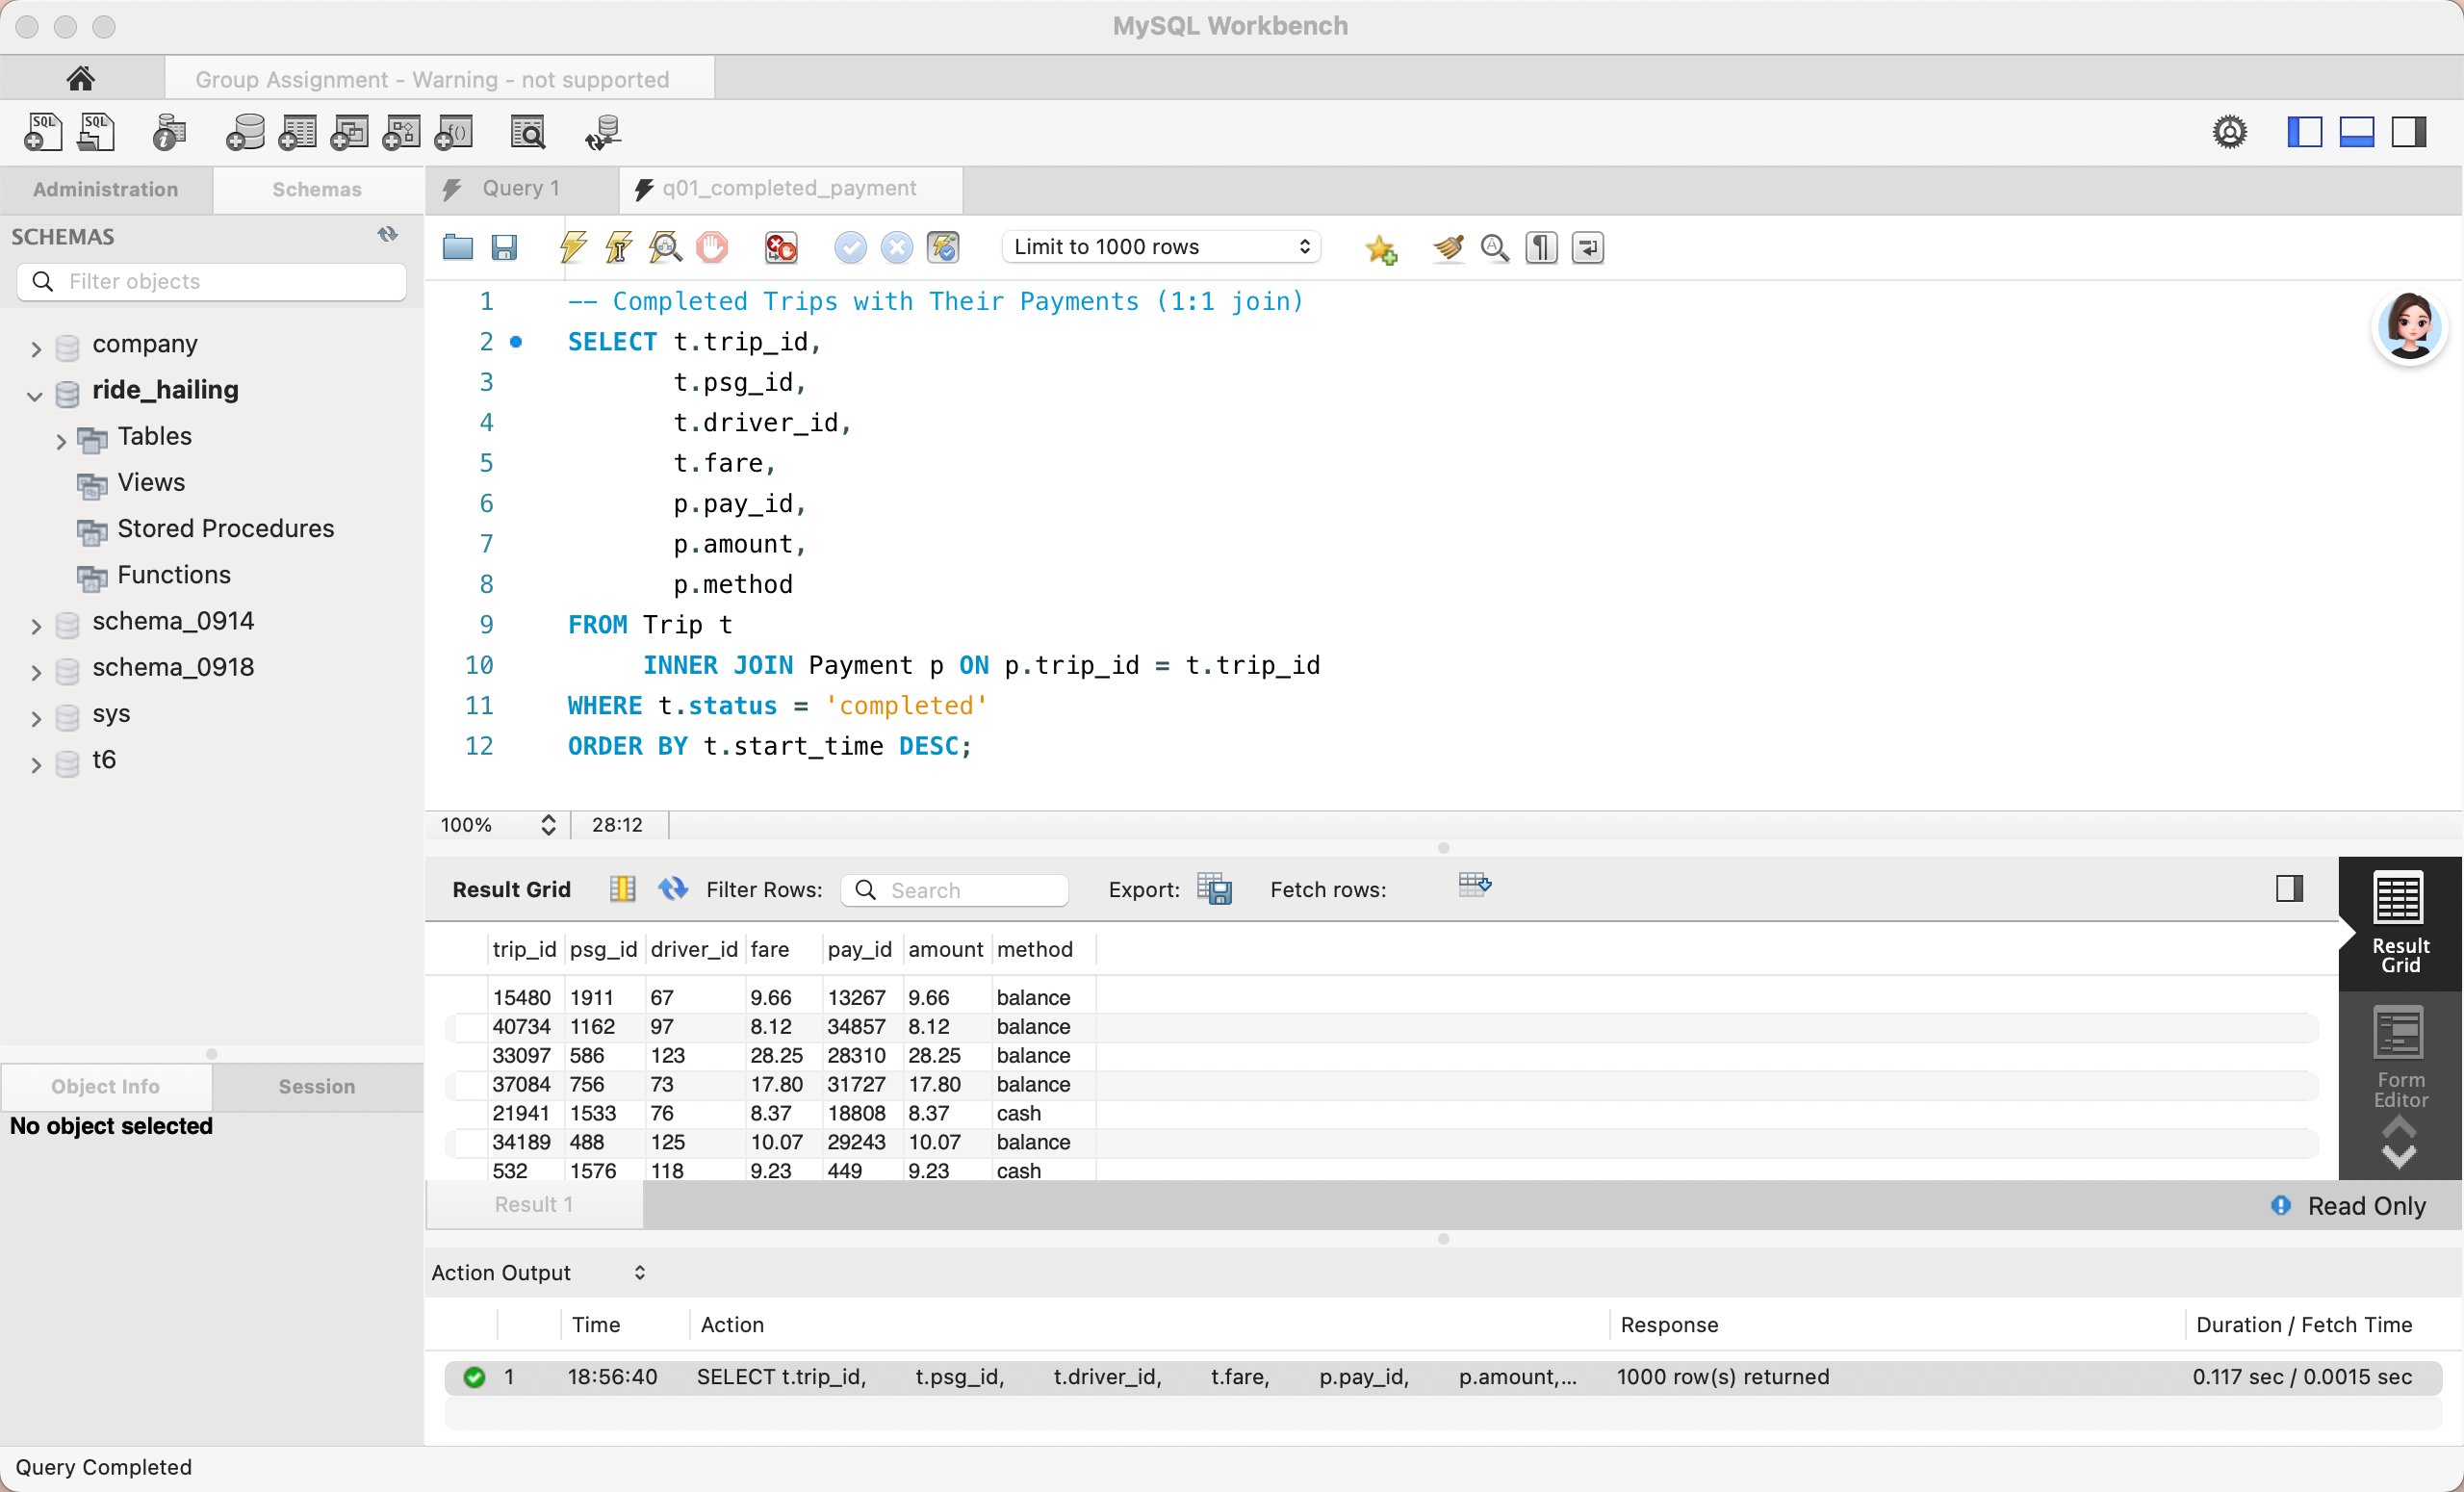
\includegraphics[width=0.72\textwidth]{q01_completed_payment_1029.png}
\caption{Q1 result (first 1{,}000 rows shown; full set $\approx$49.2k completed--paid pairs).}\label{fig:q01}
\end{figure}

\paragraph{Q2: Drivers with completed but unpaid trips.}
The collections list. A \texttt{NOT EXISTS} anti-join keeps exactly those completed trips that have no Payment row; \texttt{DISTINCT} collapses them to the driver level. Note the scope: cancelled trips with the \$1.50 fee already carry exactly one Payment (design decision D-06) and are therefore outside this list --- this query targets genuinely uncollected completed fares.

\begin{lstlisting}[caption={Q2 --- completed but unpaid drivers (NOT EXISTS).}]
SELECT DISTINCT d.driver_id, d.name
FROM Driver d
     INNER JOIN Trip t ON t.driver_id = d.driver_id
WHERE t.status = 'completed'
      AND NOT EXISTS (SELECT 1
                       FROM Payment p
                       WHERE p.trip_id = t.trip_id)
ORDER BY d.driver_id;
\end{lstlisting}

\begin{figure}[h]\centering
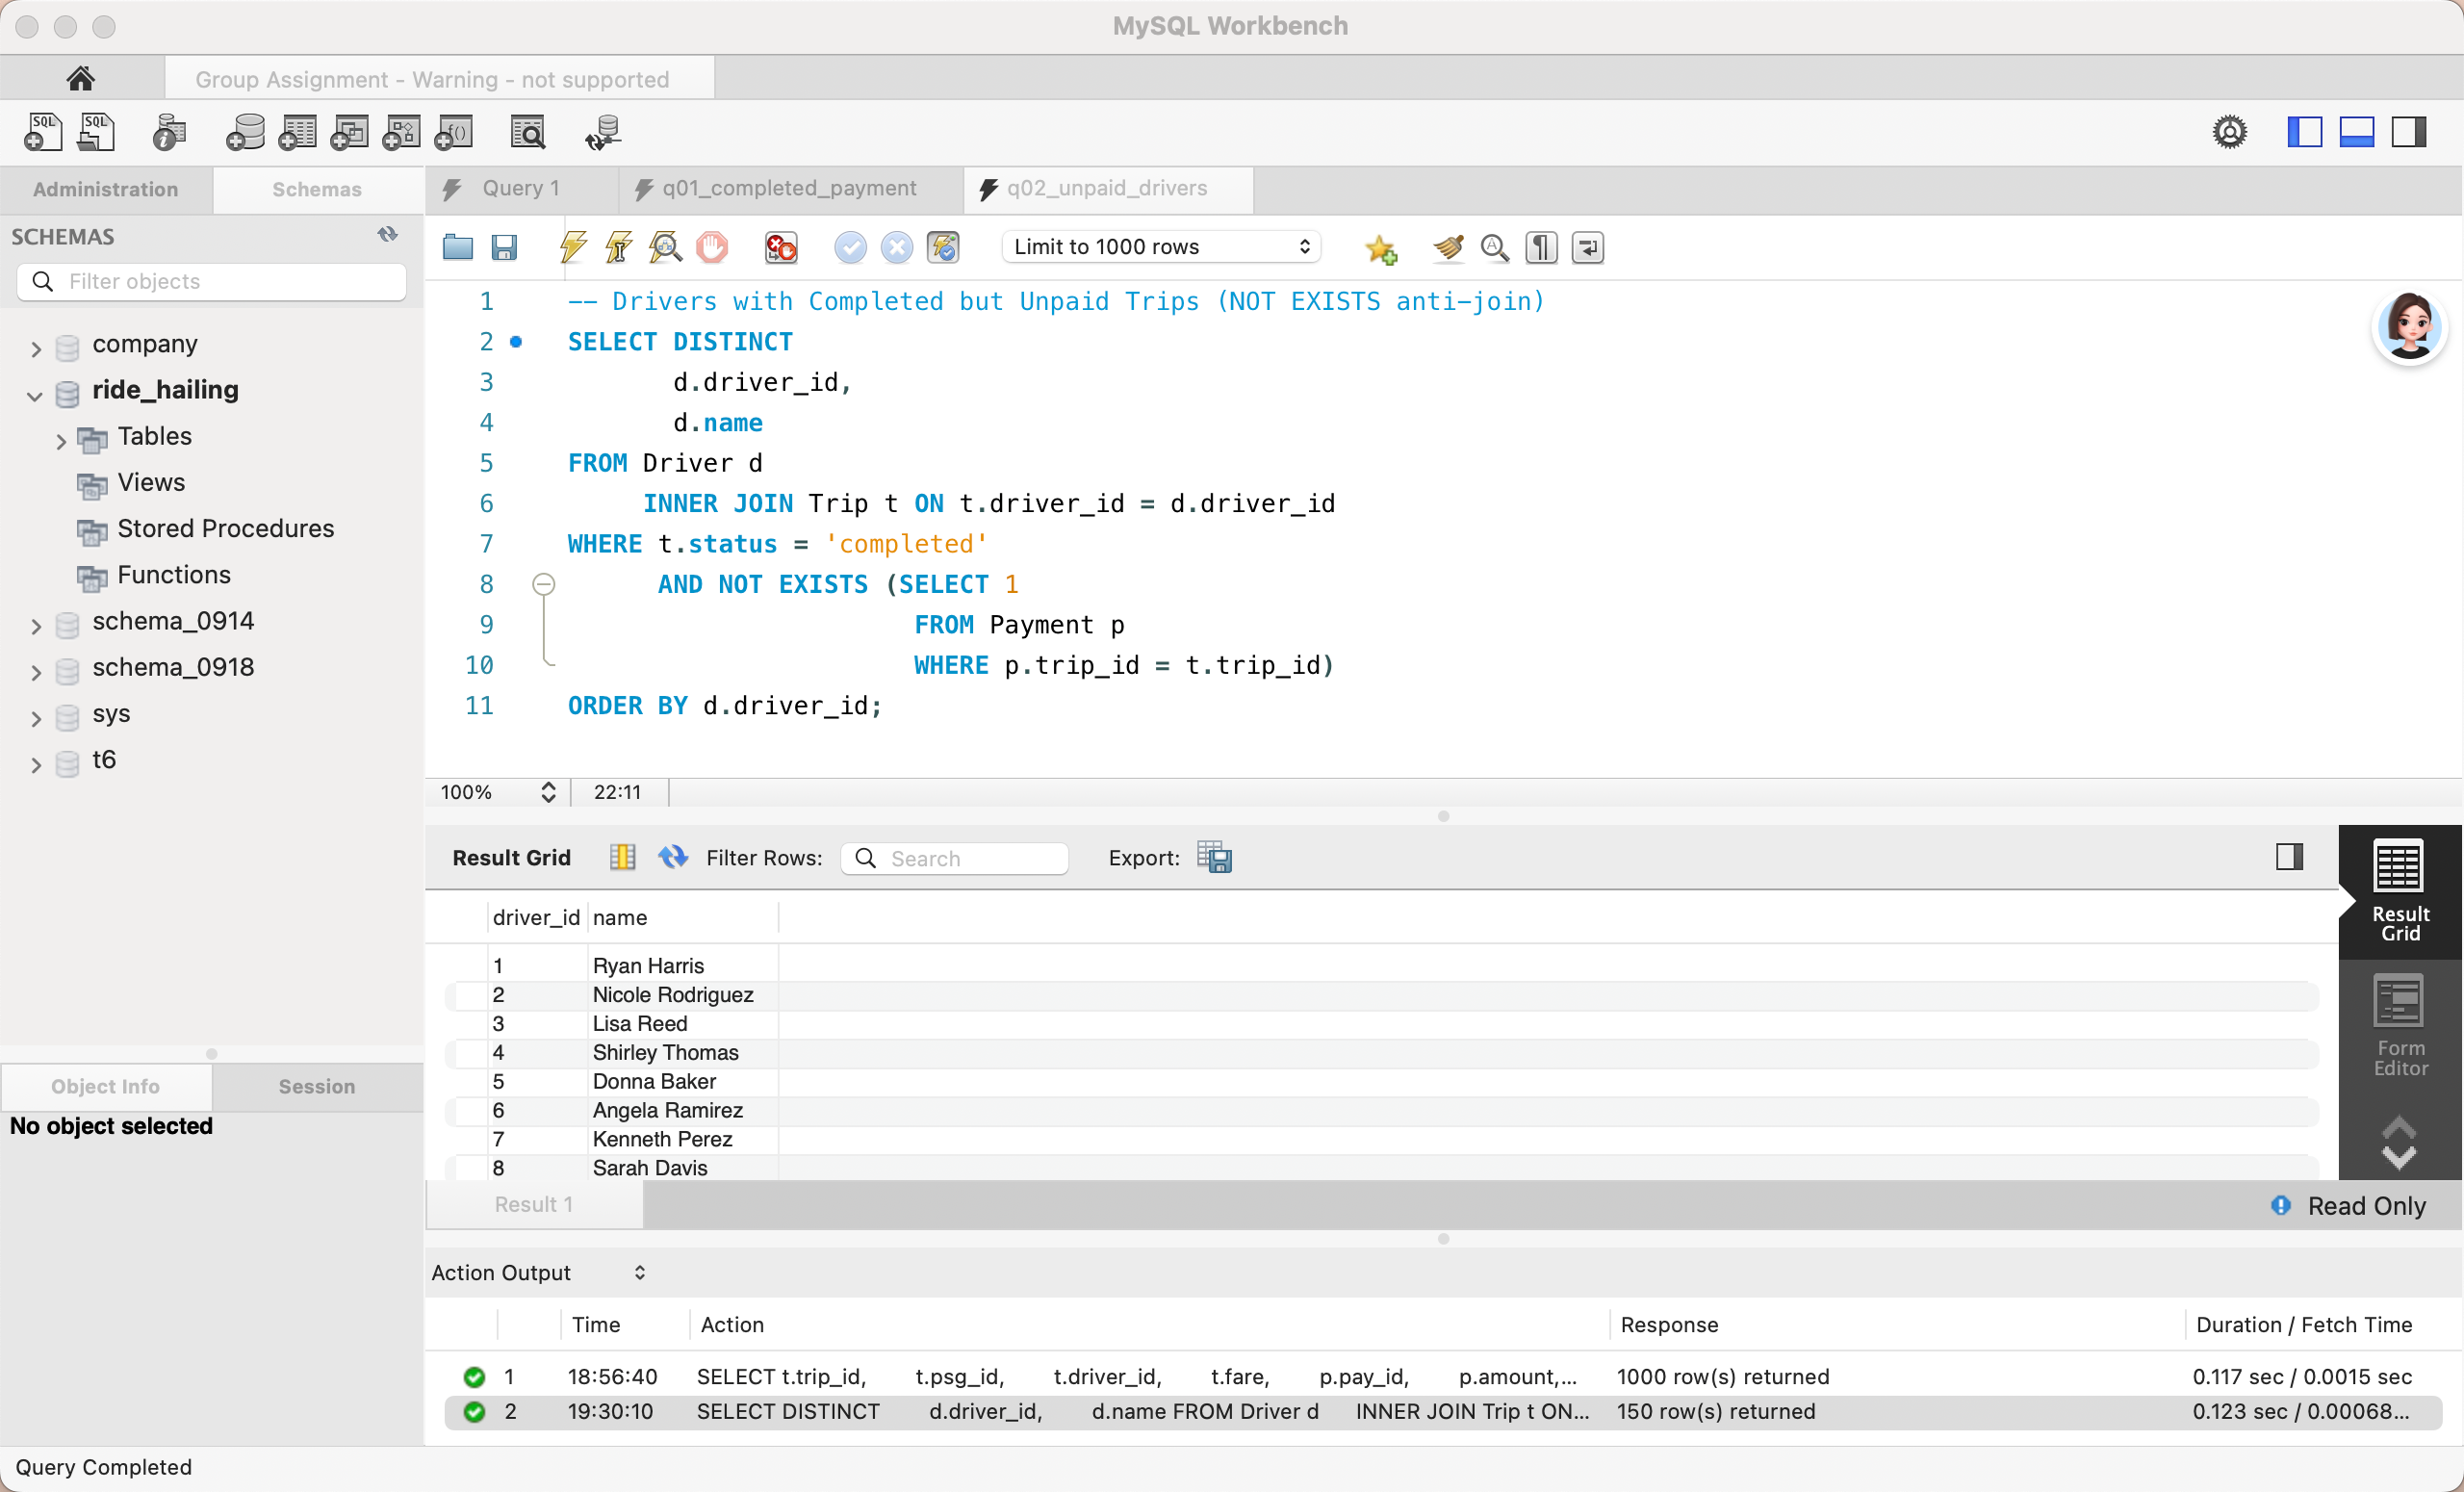
\includegraphics[width=0.72\textwidth]{q02_unpaid_drivers_1029.png}
\caption{Q2 result: all 150 drivers carry some unpaid completed trips (1{,}442 in total, by design $\approx$2.9\%).}\label{fig:q02}
\end{figure}

\paragraph{Q3: Total fare per vehicle.}
The asset-level accounting view across \texttt{Vehicle} $\to$ \texttt{Driver} $\to$ \texttt{Trip}. Revenue is well balanced --- head vehicles accumulate roughly 440--460 trips against a fleet average of 400 --- so no single asset dominates, which supports stable per-vehicle reporting.

\begin{lstlisting}[caption={Q3 --- total fare per vehicle (3-table join).}]
SELECT v.plate,
       ROUND(SUM(t.fare), 2) AS total_fare,
       COUNT(*) AS trip_cnt
FROM Vehicle v
     INNER JOIN Driver d ON d.vehicle_id = v.vehicle_id
     INNER JOIN Trip   t ON t.driver_id  = d.driver_id
GROUP BY v.vehicle_id, v.plate
ORDER BY total_fare DESC;
\end{lstlisting}

\begin{figure}[h]\centering
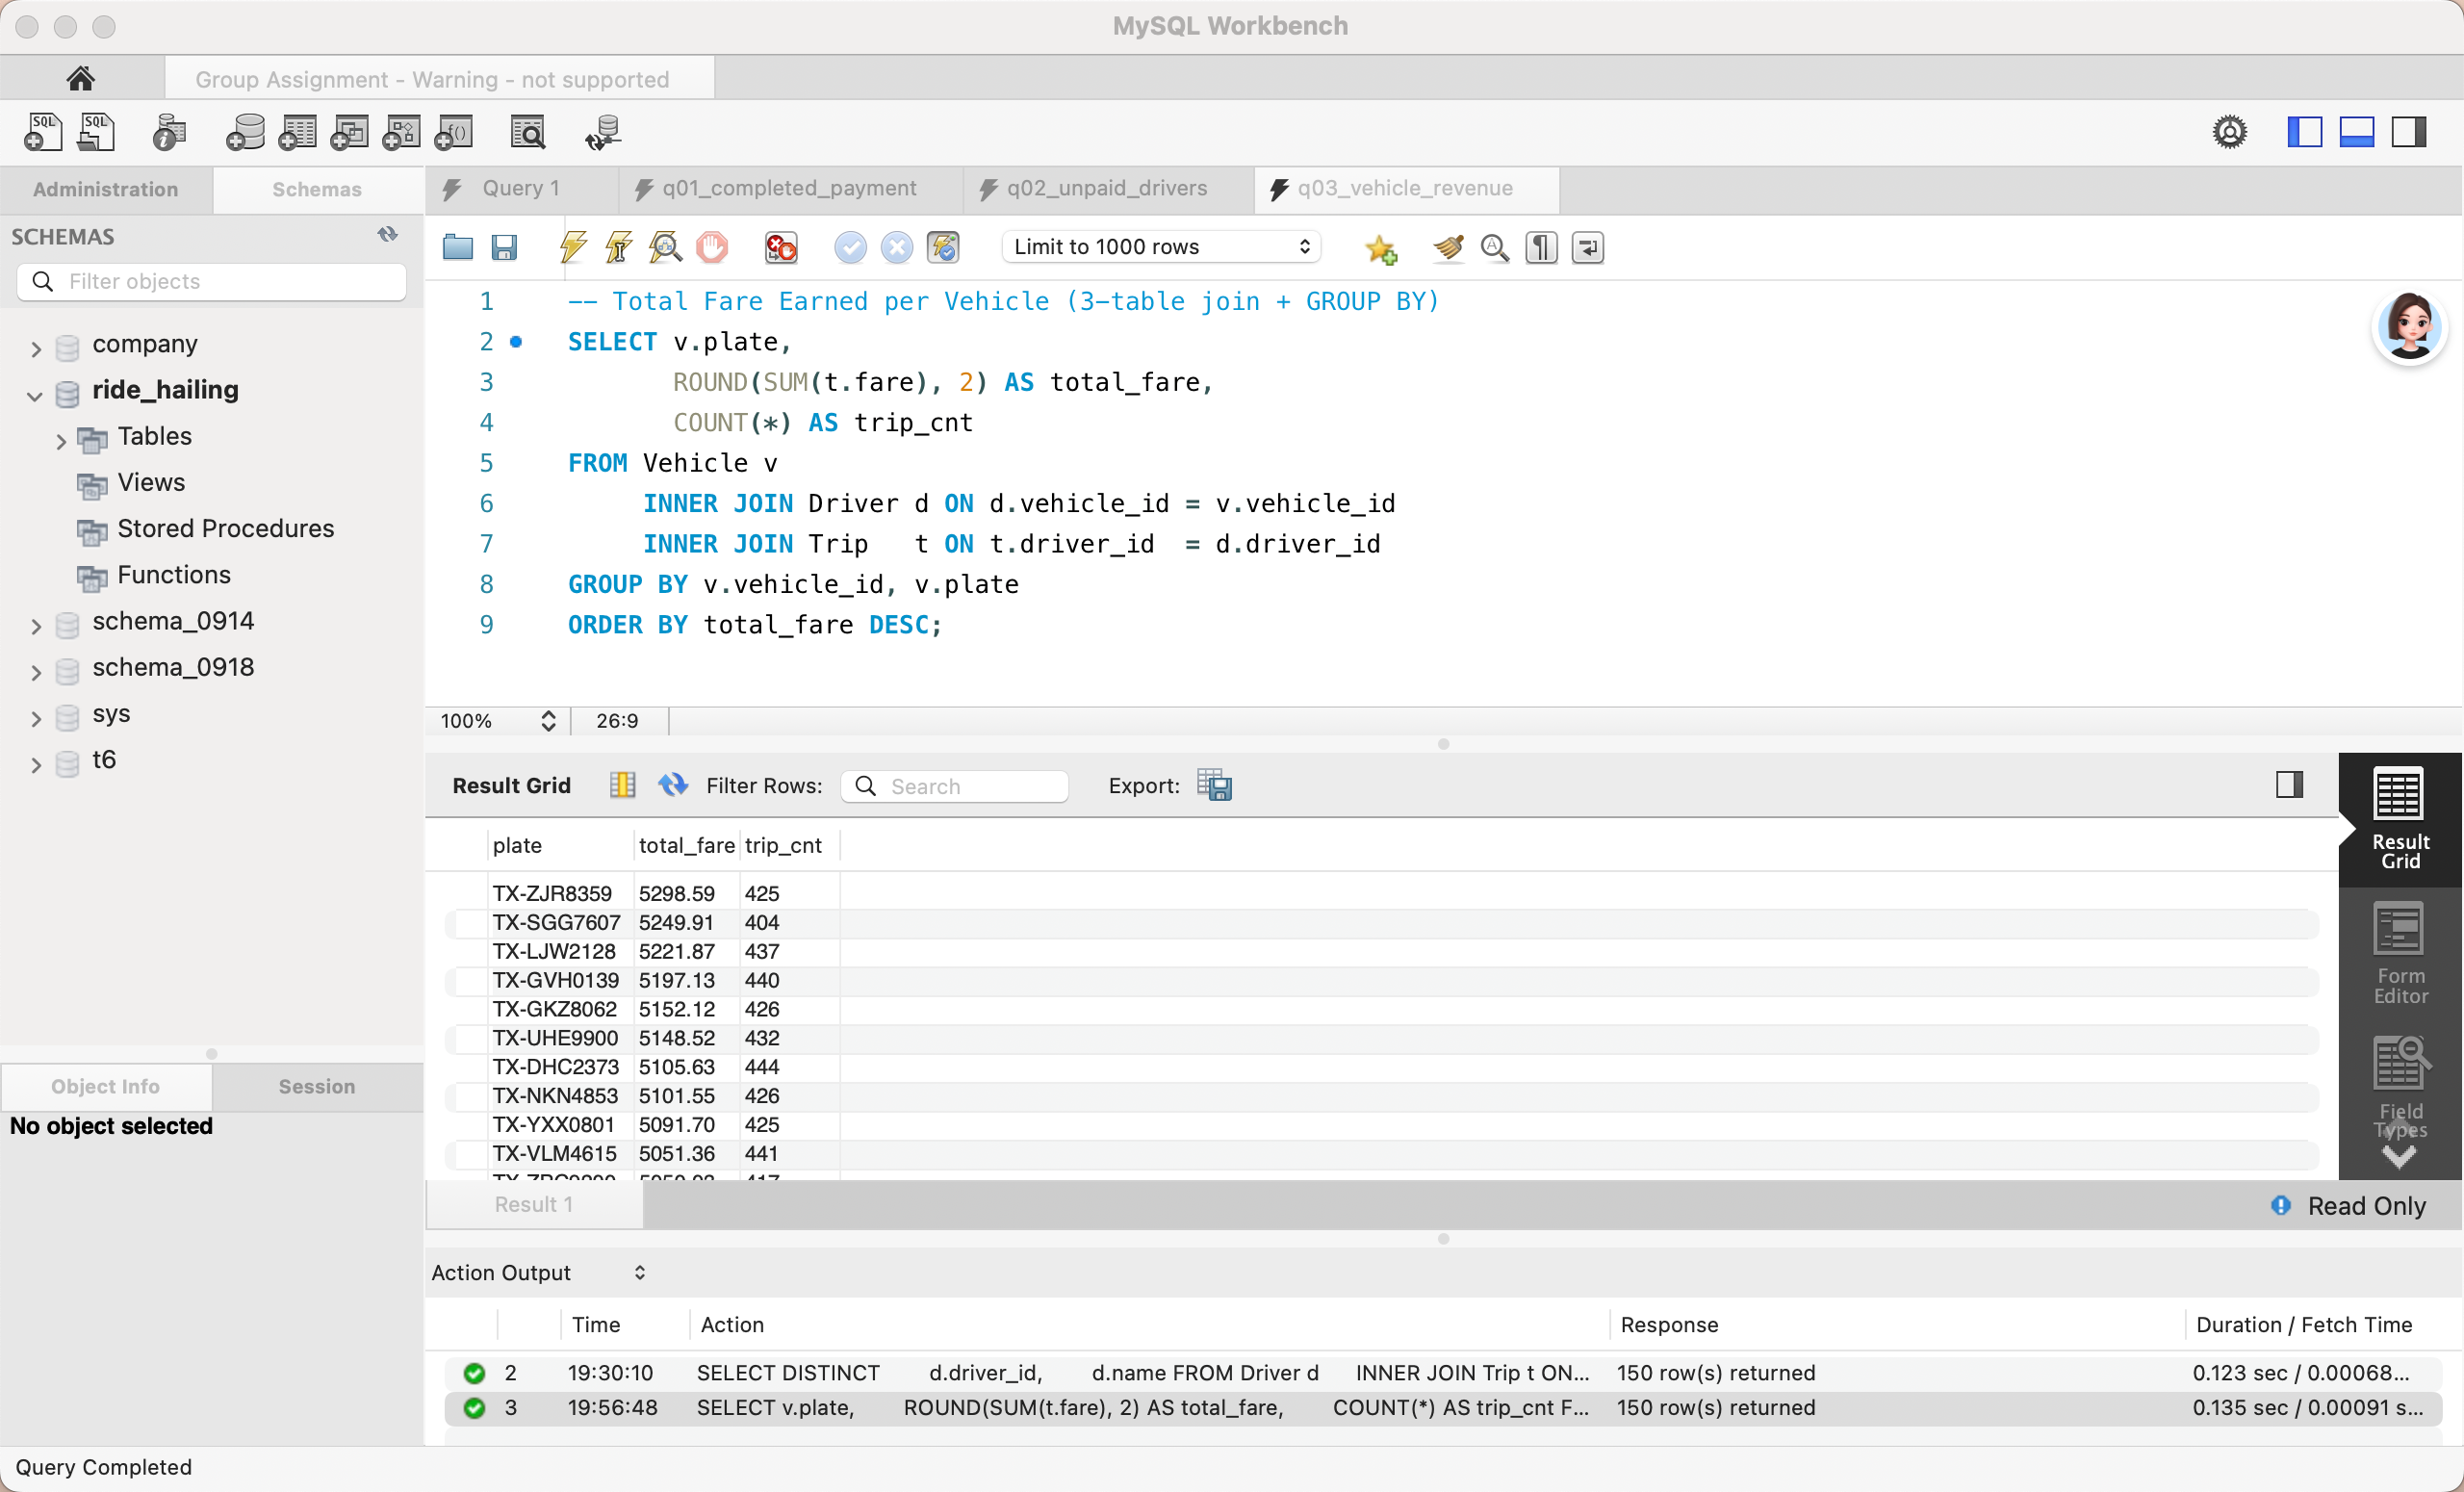
\includegraphics[width=0.72\textwidth]{q03_vehicle_revenue_1029.png}
\caption{Q3 result over the 150-vehicle fleet.}\label{fig:q03}
\end{figure}

\paragraph{Q4: Driver daily income ranking.}
Finds the ``driver of the day''. The derived table aggregates per driver and day first; the window function \texttt{RANK() OVER (ORDER BY day\_income DESC)} then ranks the aggregated rows in a single pass, avoiding a self-join formulation. The top driver-day earns \$292, well above a typical day, showing how earnings concentrate on peak days.

\begin{lstlisting}[caption={Q4 --- driver daily income ranking (window function).}]
SELECT driver_id, income_date, day_income,
       RANK() OVER (ORDER BY day_income DESC) AS rnk
FROM (SELECT driver_id,
              DATE(start_time) AS income_date,
              ROUND(SUM(fare), 2) AS day_income
       FROM Trip
       WHERE status = 'completed'
       GROUP BY driver_id, DATE(start_time)) AS daily
ORDER BY rnk
LIMIT 10;
\end{lstlisting}

\begin{figure}[h]\centering
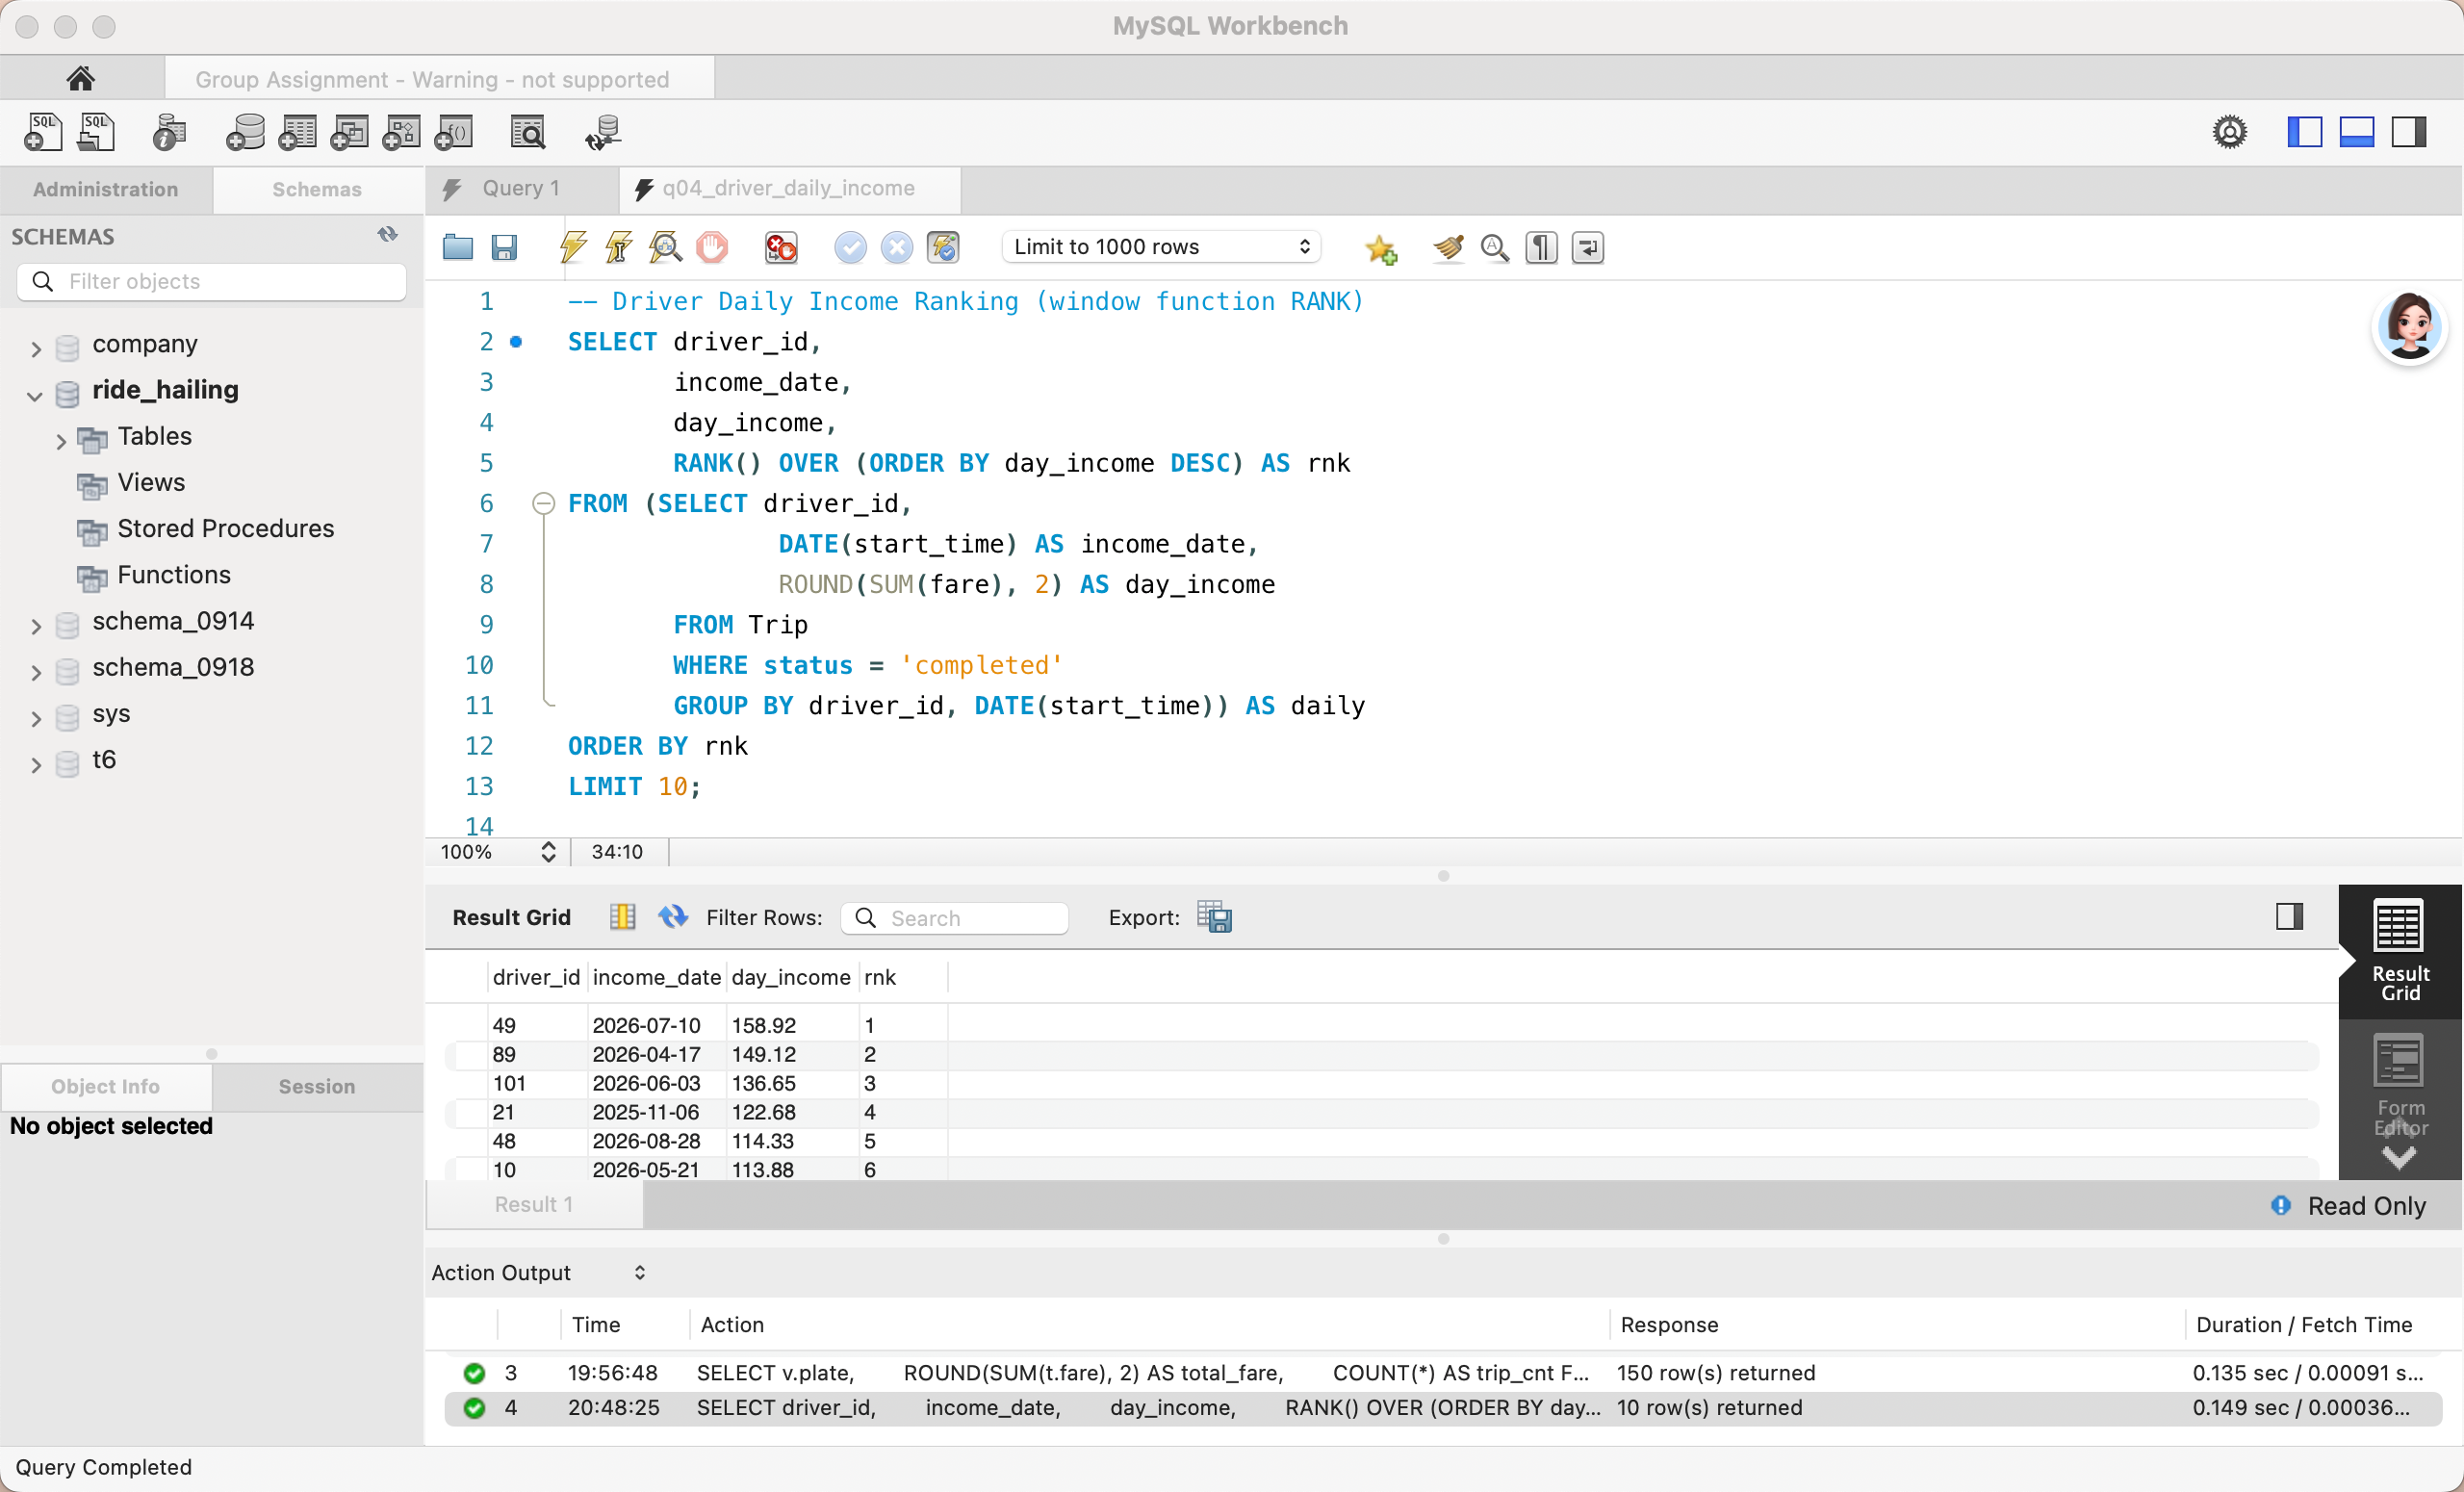
\includegraphics[width=0.72\textwidth]{q04_driver_daily_income_1029.png}
\caption{Q4 result: top-10 driver-days.}\label{fig:q04}
\end{figure}

\paragraph{Q5: Completed trips unpaid for over 24 hours.}
The receivables exposure view. Because the simulated history ends before load time, every one of the 1{,}442 unpaid completed trips is already far beyond the threshold, so the filter currently passes all of them and the exposure equals the sum of their fares; in production the same threshold would isolate genuinely overdue receivables.

\begin{lstlisting}[caption={Q5 --- unpaid $>$24h (anti-join + time filter).}]
SELECT t.trip_id, t.driver_id, t.fare, t.start_time,
       TIMESTAMPDIFF(HOUR, t.start_time, NOW()) AS hours_unpaid
FROM Trip t
WHERE t.status = 'completed'
      AND t.start_time < NOW() - INTERVAL 24 HOUR
      AND NOT EXISTS (SELECT 1 FROM Payment p WHERE p.trip_id = t.trip_id)
ORDER BY hours_unpaid DESC;
\end{lstlisting}

\begin{figure}[h]\centering
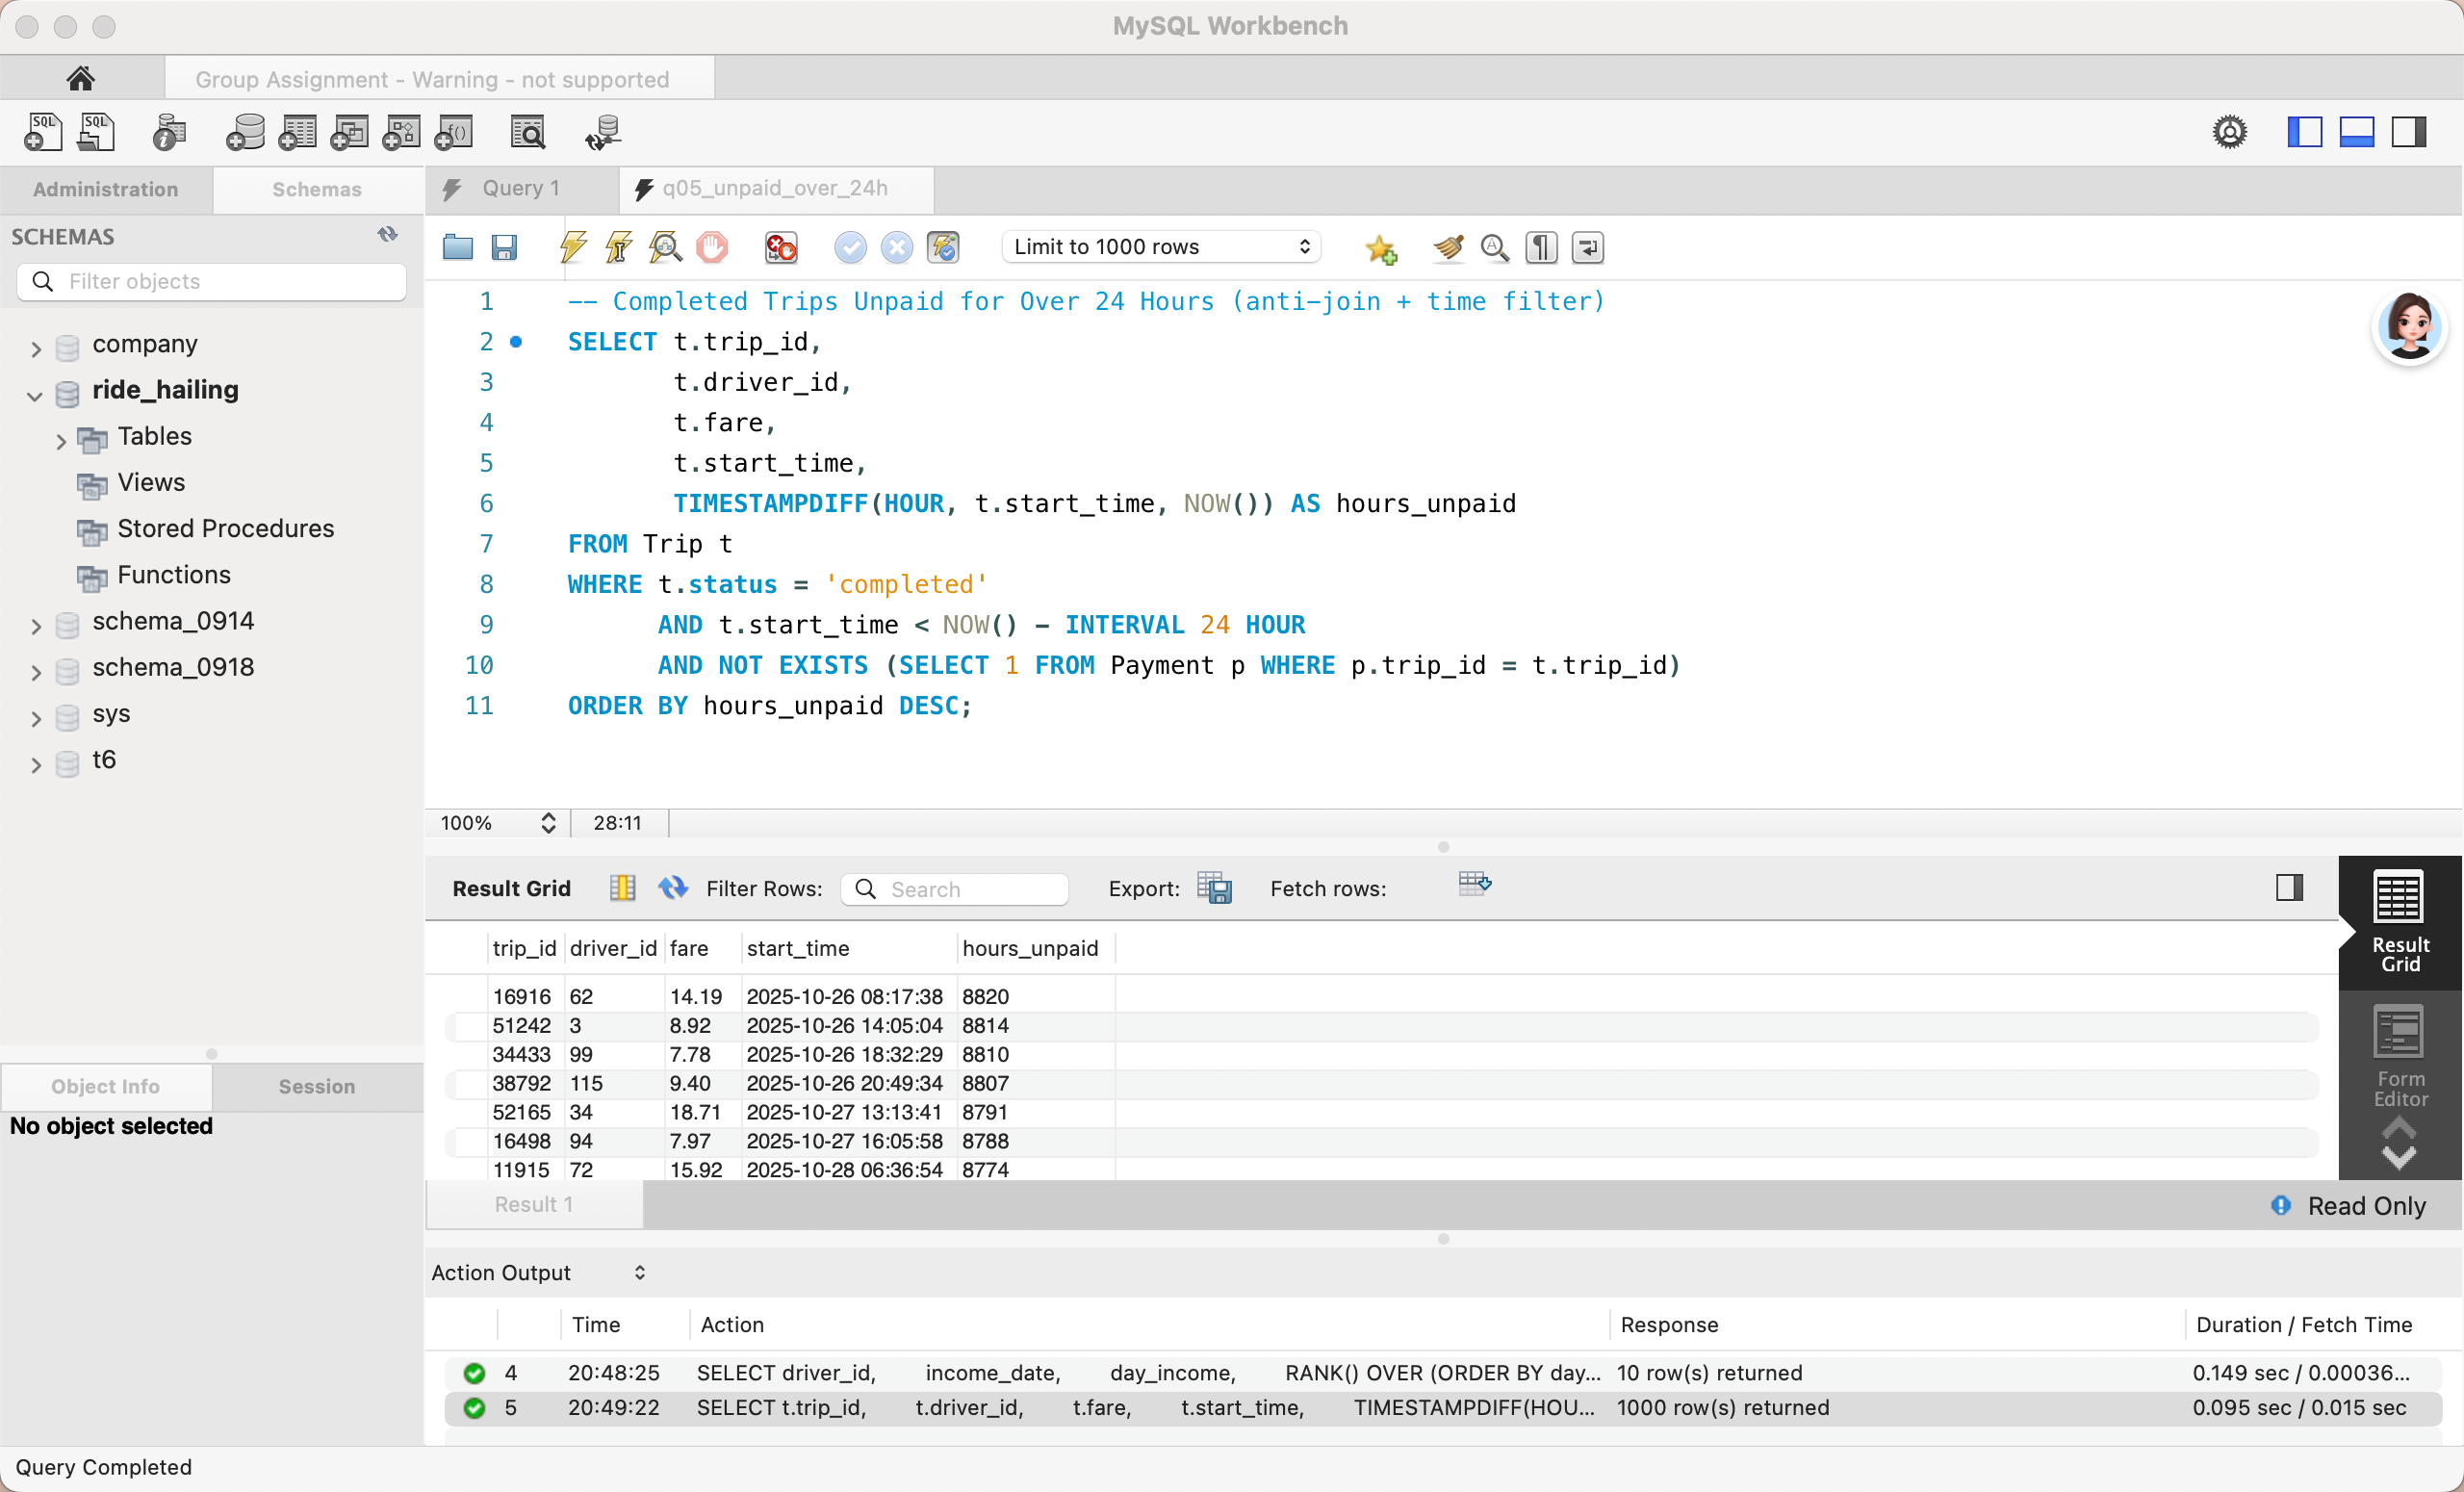
\includegraphics[width=0.72\textwidth]{q05_unpaid_over_24h_1029.png}
\caption{Q5 result (first 1{,}000 of 1{,}442 rows shown).}\label{fig:q05}
\end{figure}

\paragraph{Q6: Peak-hour order volume.}
Groups all accepted trips by hour of day and keeps only hours reaching the 2{,}000-trip threshold --- a \texttt{HAVING} filter over groups that \texttt{WHERE} could never express. Demand concentrates in the evening block 17:00--20:00 (13{,}459 trips, 22.4\% of accepted volume) with a secondary morning shoulder, peaking at 3{,}915 trips in hour 18; dispatch should pre-position supply before 17:00.

\begin{lstlisting}[caption={Q6 --- peak-hour volume (GROUP BY + HAVING).}]
SELECT HOUR(start_time) AS hr,
       COUNT(*) AS trips
FROM Trip
GROUP BY HOUR(start_time)
HAVING COUNT(*) >= 2000
ORDER BY trips DESC;
\end{lstlisting}

\begin{figure}[h]\centering
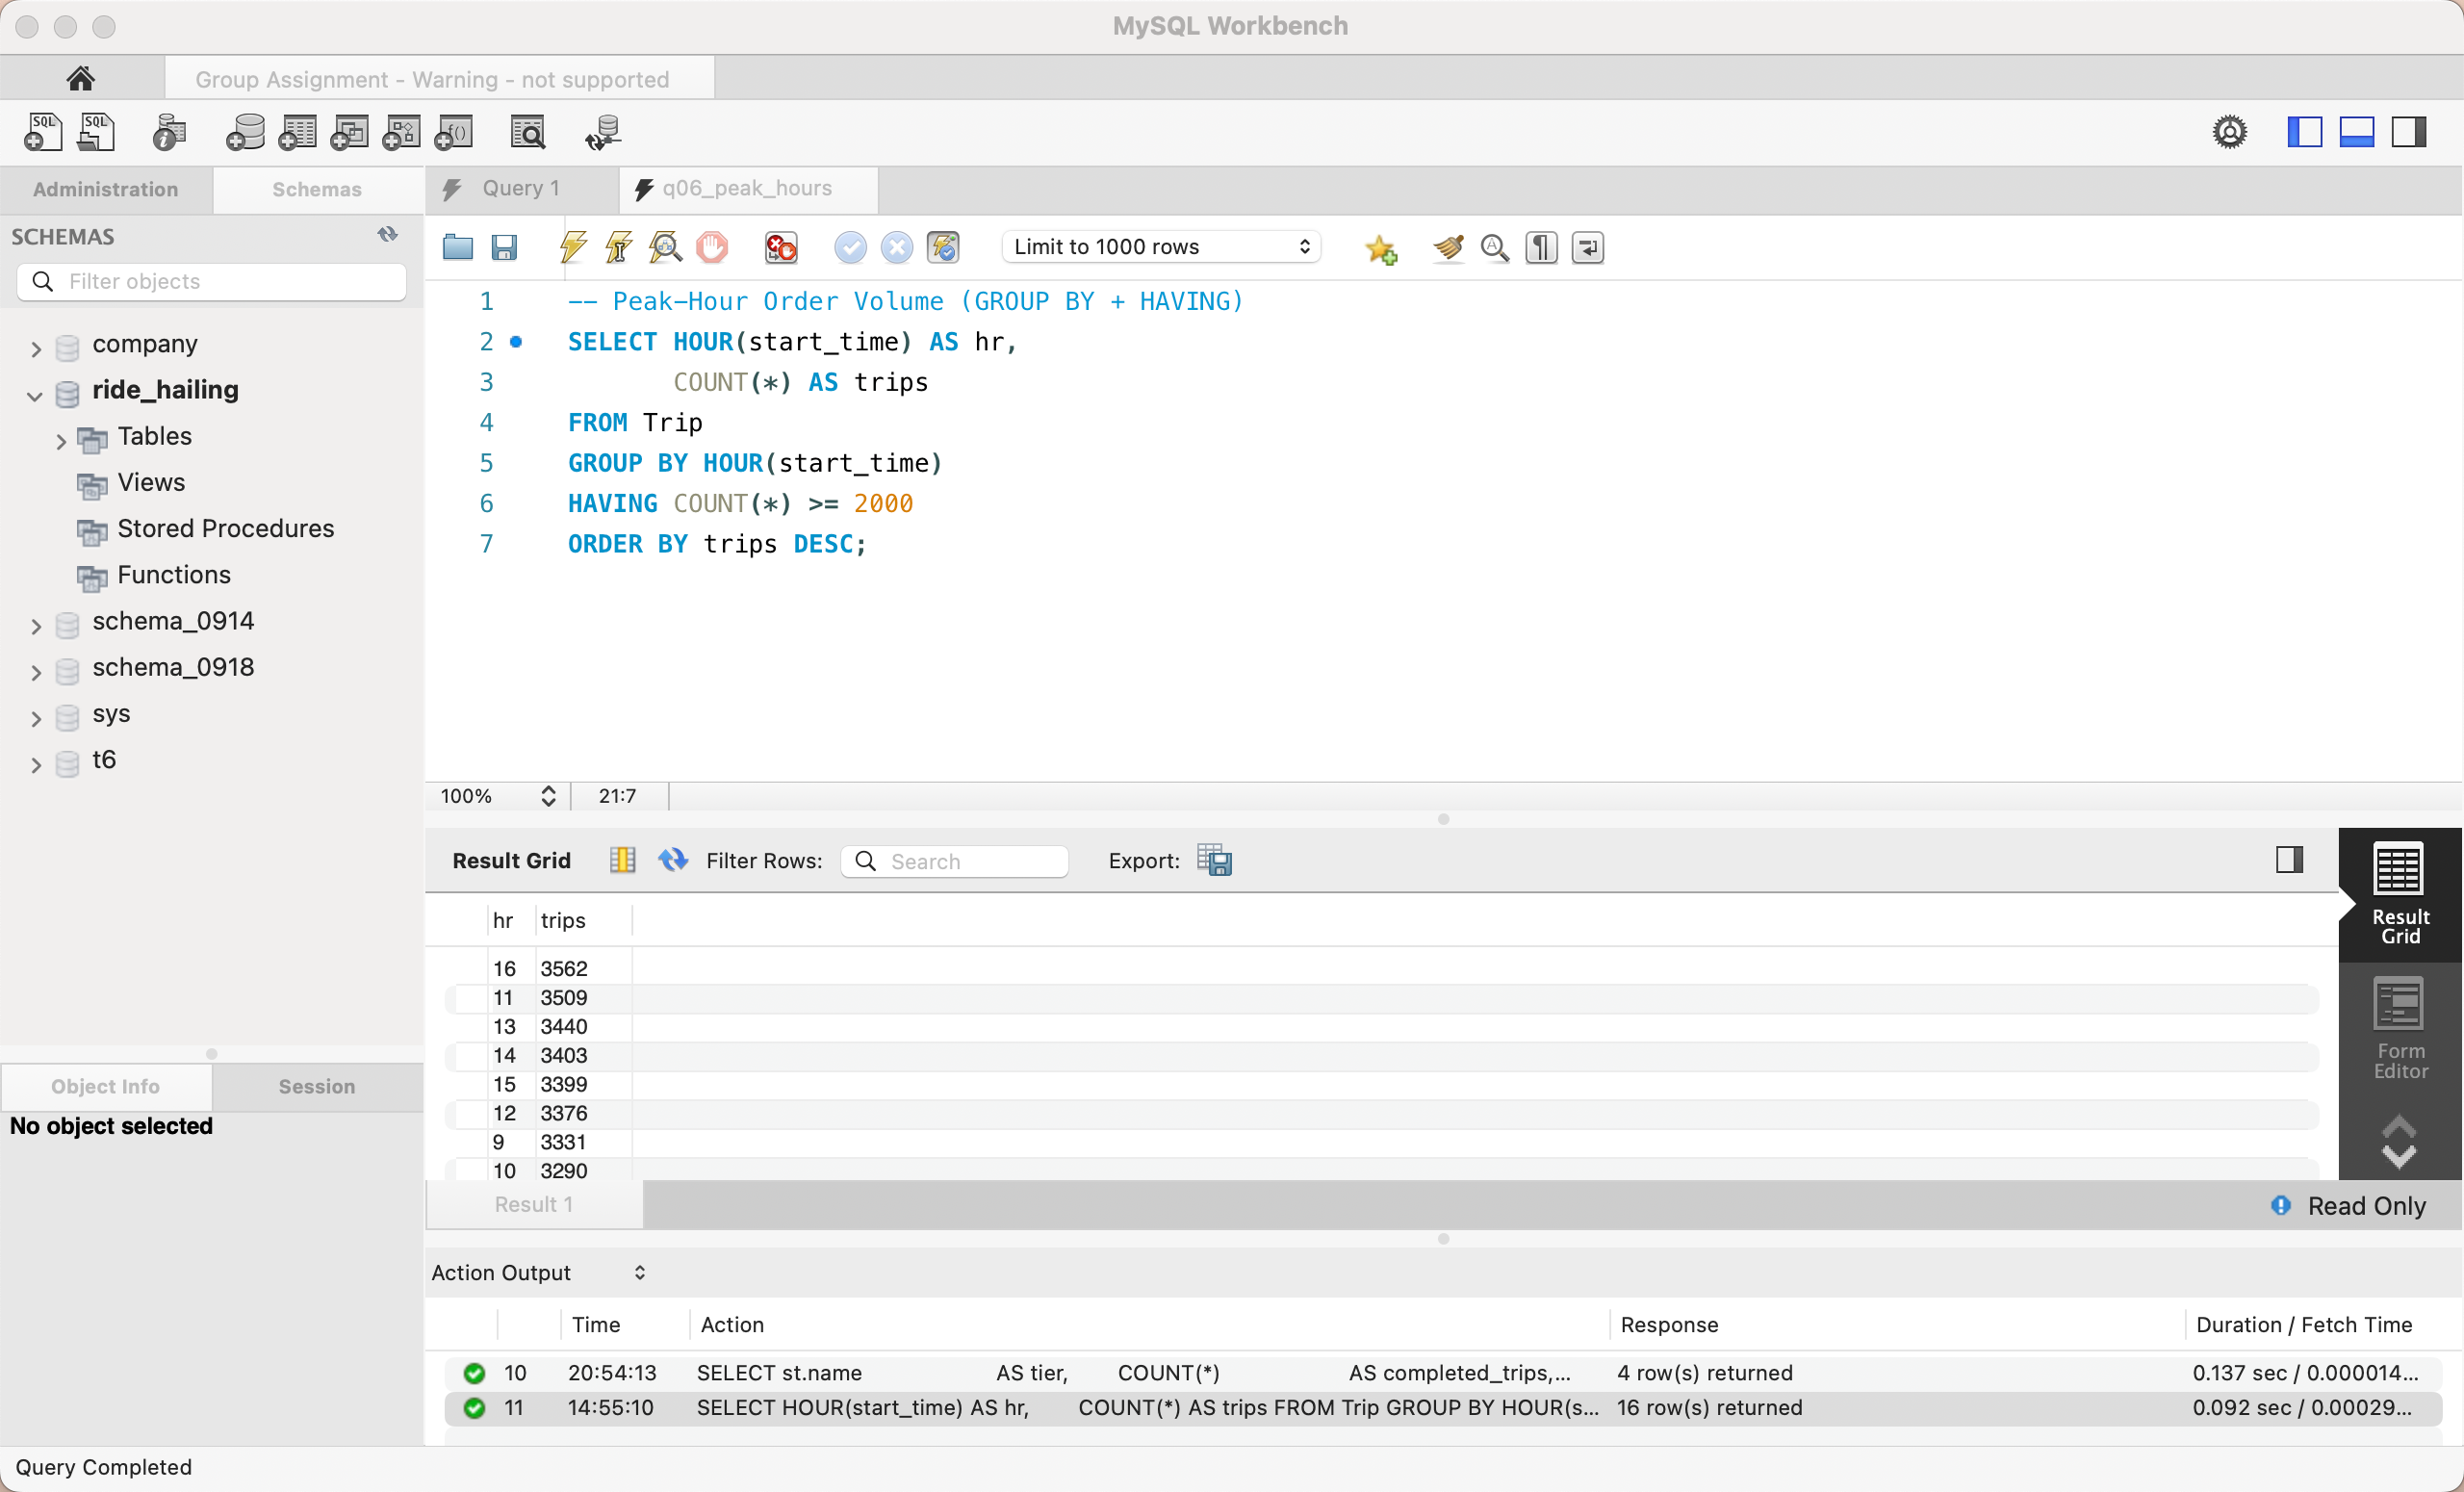
\includegraphics[width=0.72\textwidth]{q06_peak_hours_1029.png}
\caption{Q6 result: 14 hours exceed the 2{,}000-trip threshold.}\label{fig:q06}
\end{figure}

\paragraph{Q7: Monthly revenue trend.}
Joins payments back to trip start months for the GMV view. Paid revenue rises steadily from \$49.3k (2025-11) to \$54.8k (2026-10), about +11\% over twelve months with no seasonal dip, supporting the growth assumption stated in Section~\ref{sec:context}.

\begin{lstlisting}[caption={Q7 --- monthly revenue trend.}]
SELECT DATE_FORMAT(t.start_time, '%Y-%m') AS ym,
       COUNT(*) AS paid_trips,
       ROUND(SUM(p.amount), 2) AS revenue
FROM Trip t
     INNER JOIN Payment p ON p.trip_id = t.trip_id
GROUP BY DATE_FORMAT(t.start_time, '%Y-%m')
ORDER BY ym;
\end{lstlisting}

\begin{figure}[h]\centering
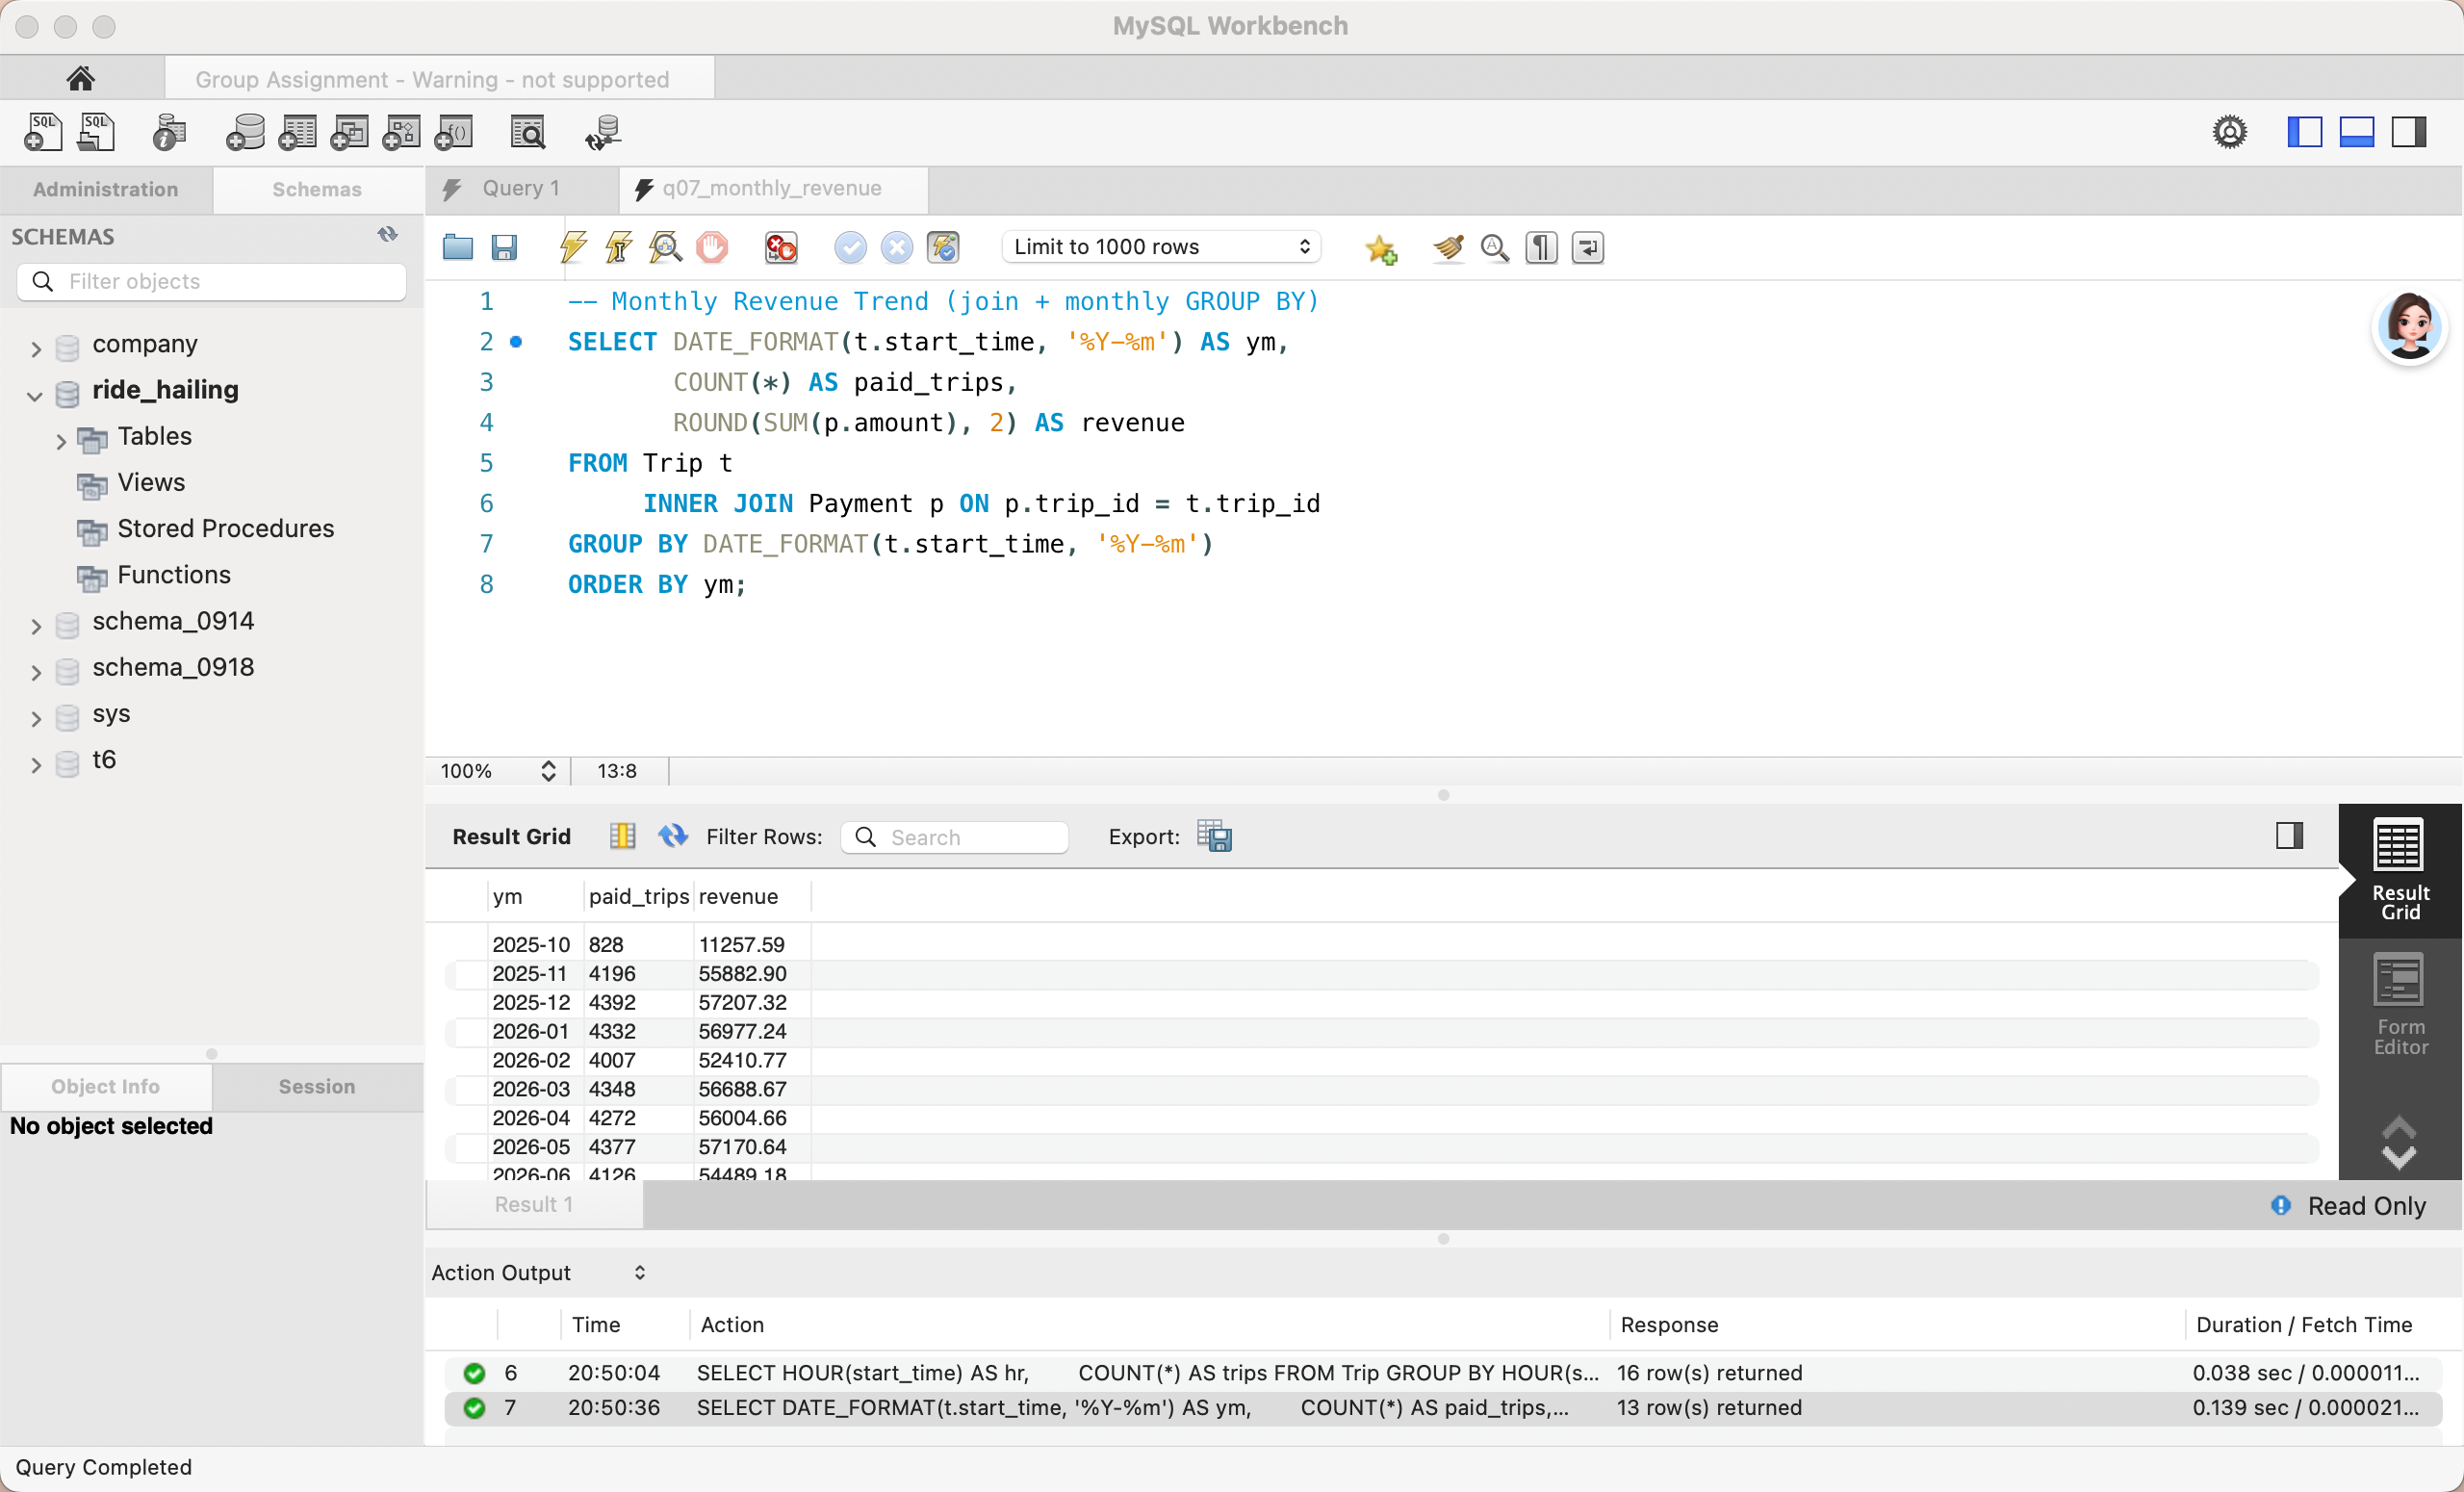
\includegraphics[width=0.72\textwidth]{q07_monthly_revenue_1029.png}
\caption{Q7 result: twelve months of paid revenue.}\label{fig:q07}
\end{figure}

\paragraph{Q8: Repeat passengers.}
Keeps passengers active on at least two distinct days. Repeat usage is the norm rather than the exception --- the list exceeds the 1{,}000-row display cap, and the heaviest passenger rides 79 trips across 74 distinct days, roughly one trip every five days; retention metrics follow directly from this pattern.

\begin{lstlisting}[caption={Q8 --- repeat passengers (COUNT DISTINCT).}]
SELECT p.psg_id, p.name,
       COUNT(*) AS total_trips,
       COUNT(DISTINCT DATE(t.start_time)) AS active_days
FROM Passenger p
     INNER JOIN Trip t ON t.psg_id = p.psg_id
GROUP BY p.psg_id, p.name
HAVING COUNT(DISTINCT DATE(t.start_time)) >= 2
ORDER BY active_days DESC, total_trips DESC;
\end{lstlisting}

\begin{figure}[h]\centering
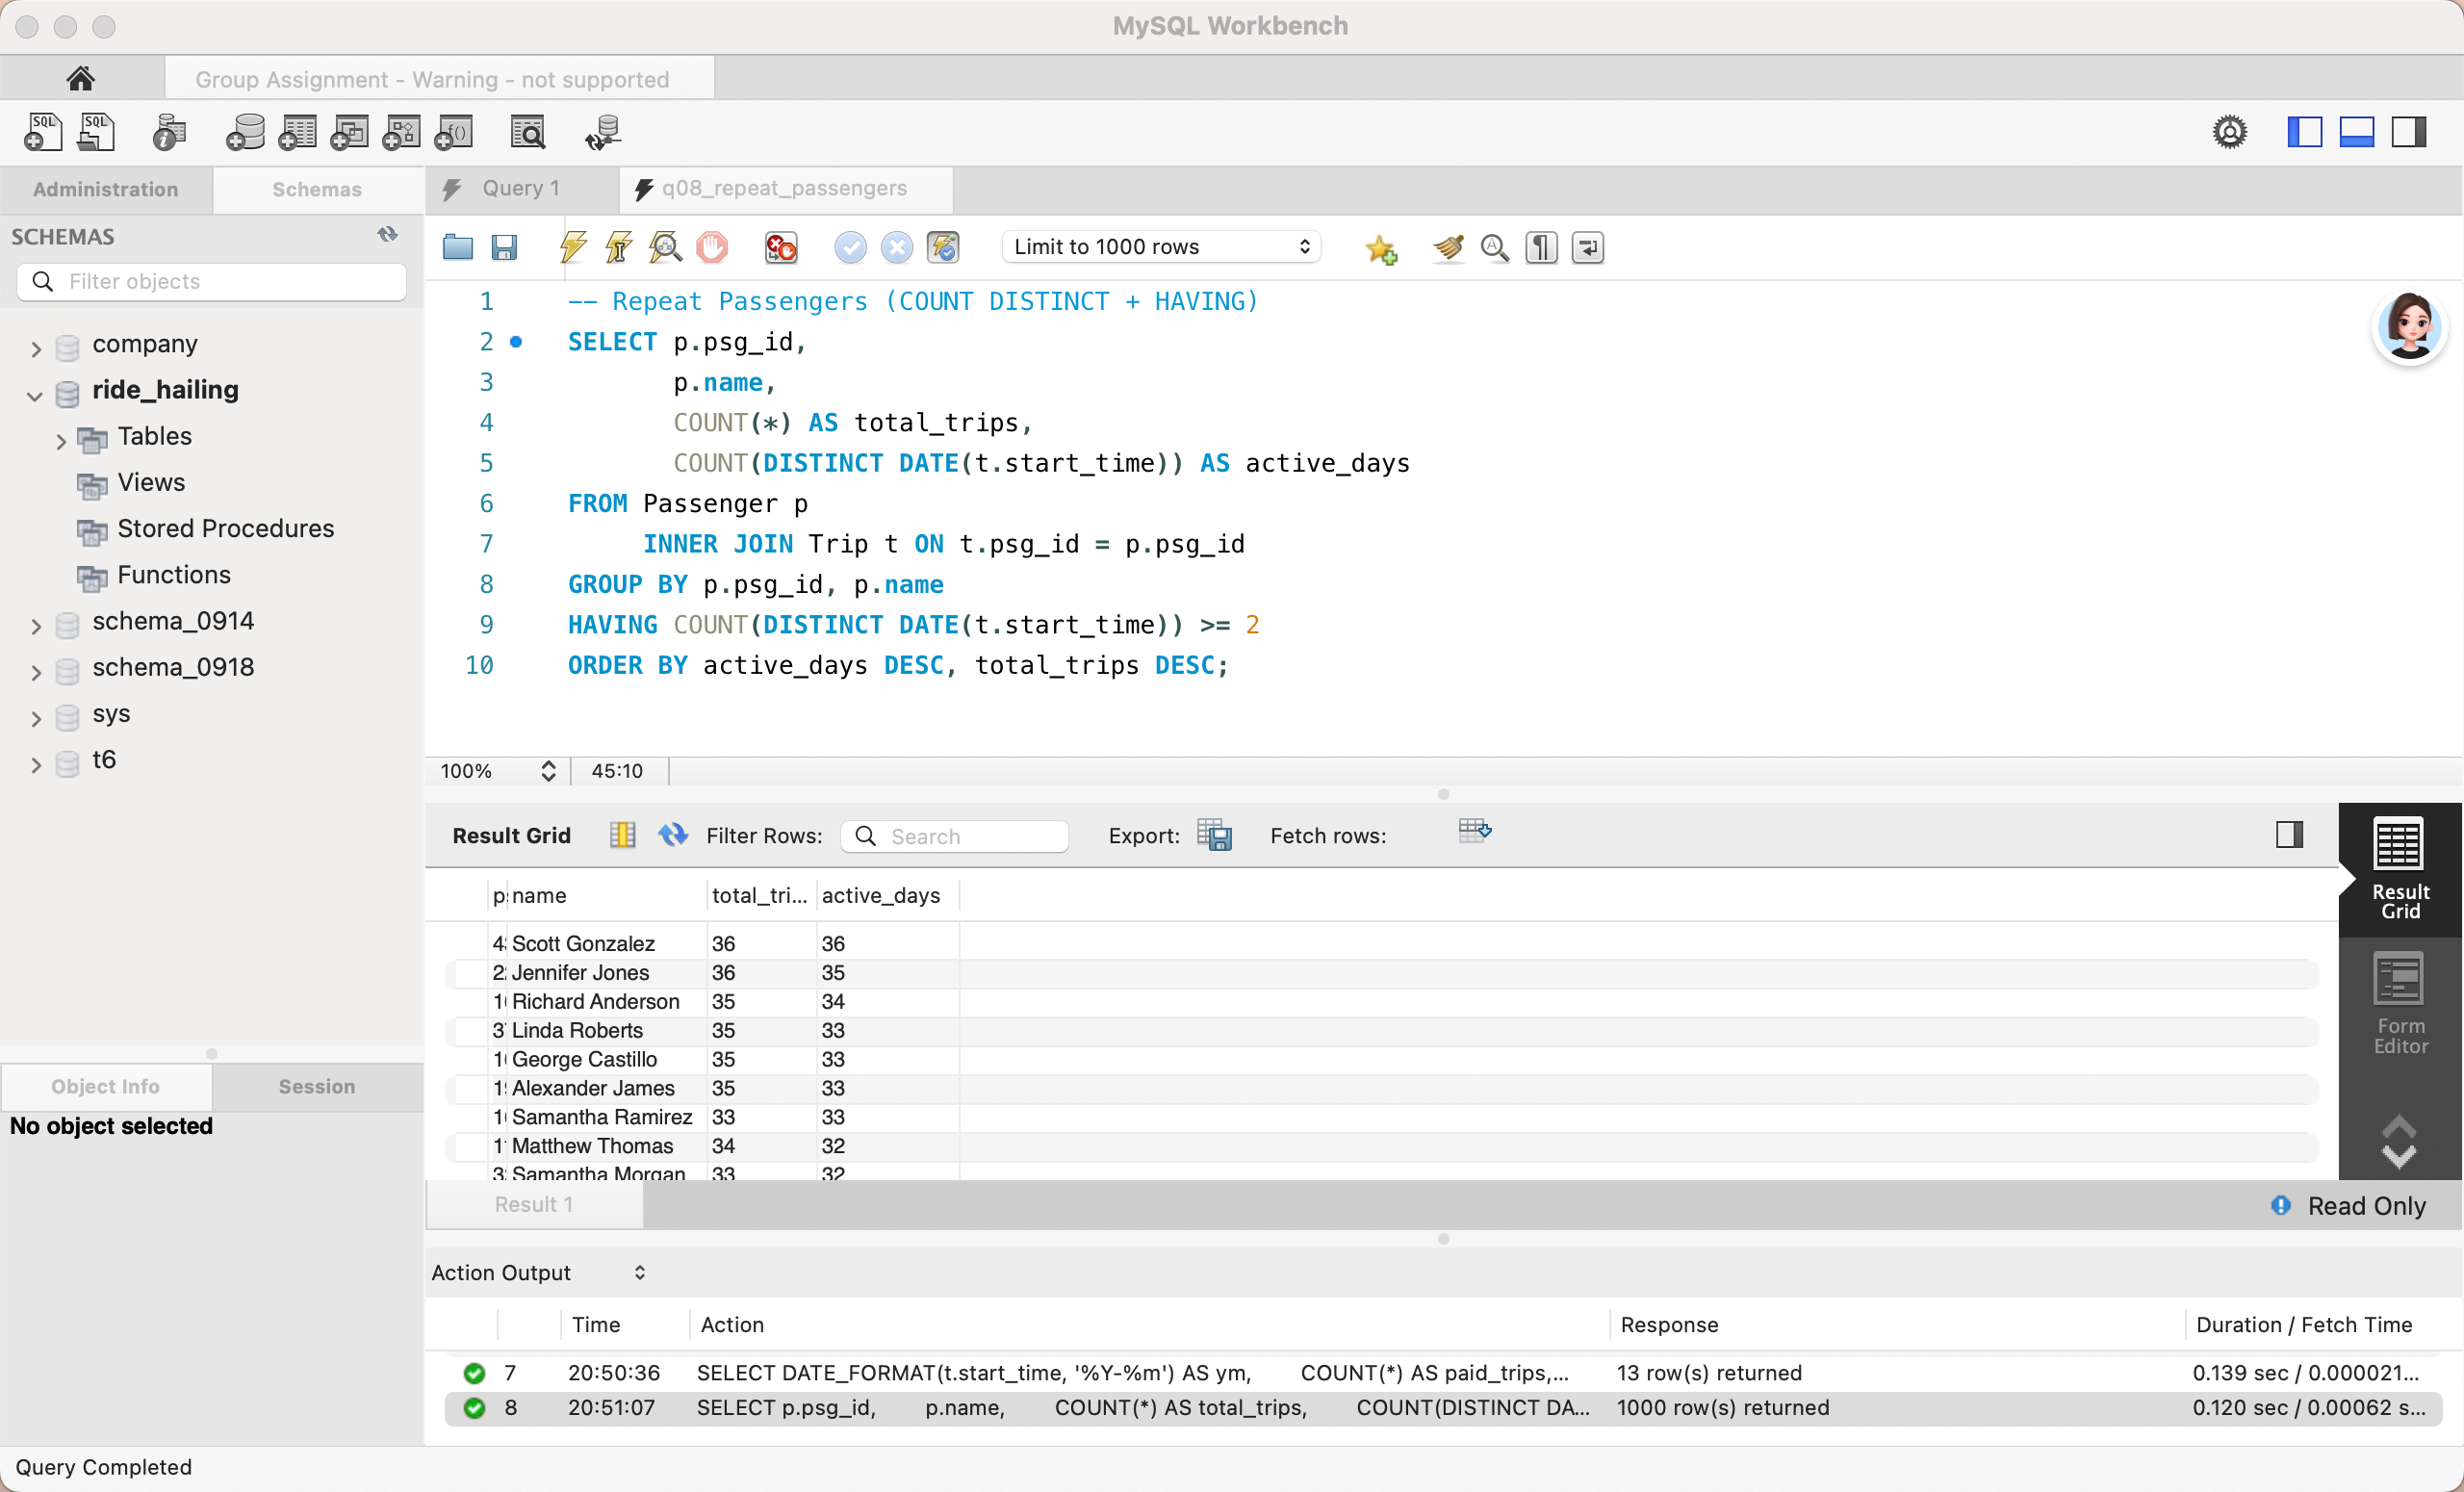
\includegraphics[width=0.72\textwidth]{q08_repeat_passengers_1029.png}
\caption{Q8 result (first 1{,}000 rows shown).}\label{fig:q08}
\end{figure}

\paragraph{Q9: Accepted trips per pickup zone.}
The spatial view enabled by the \texttt{trip\_detail} extension. The top three zones --- Downtown (16.9\%), West Campus (9.4\%) and South Congress (8.2\%) --- absorb 34.6\% of accepted trips, matching the calibrated spatial concentration of $\approx$35\%. Per decision D-11 this counts \emph{accepted} trips only: requests that never received a driver are outside the data and cannot be inferred (Section~\ref{sec:conclusion}).

\begin{lstlisting}[caption={Q9 --- accepted trips per zone (D-11 basis).}]
SELECT z.zone_id, z.name,
       COUNT(*) AS accepted_trips
FROM Trip t
     JOIN trip_detail td ON td.trip_id = t.trip_id
     JOIN pickup_zone z  ON z.zone_id   = td.zone_id
GROUP BY z.zone_id, z.name
ORDER BY accepted_trips DESC
LIMIT 15;
\end{lstlisting}

\begin{figure}[h]\centering
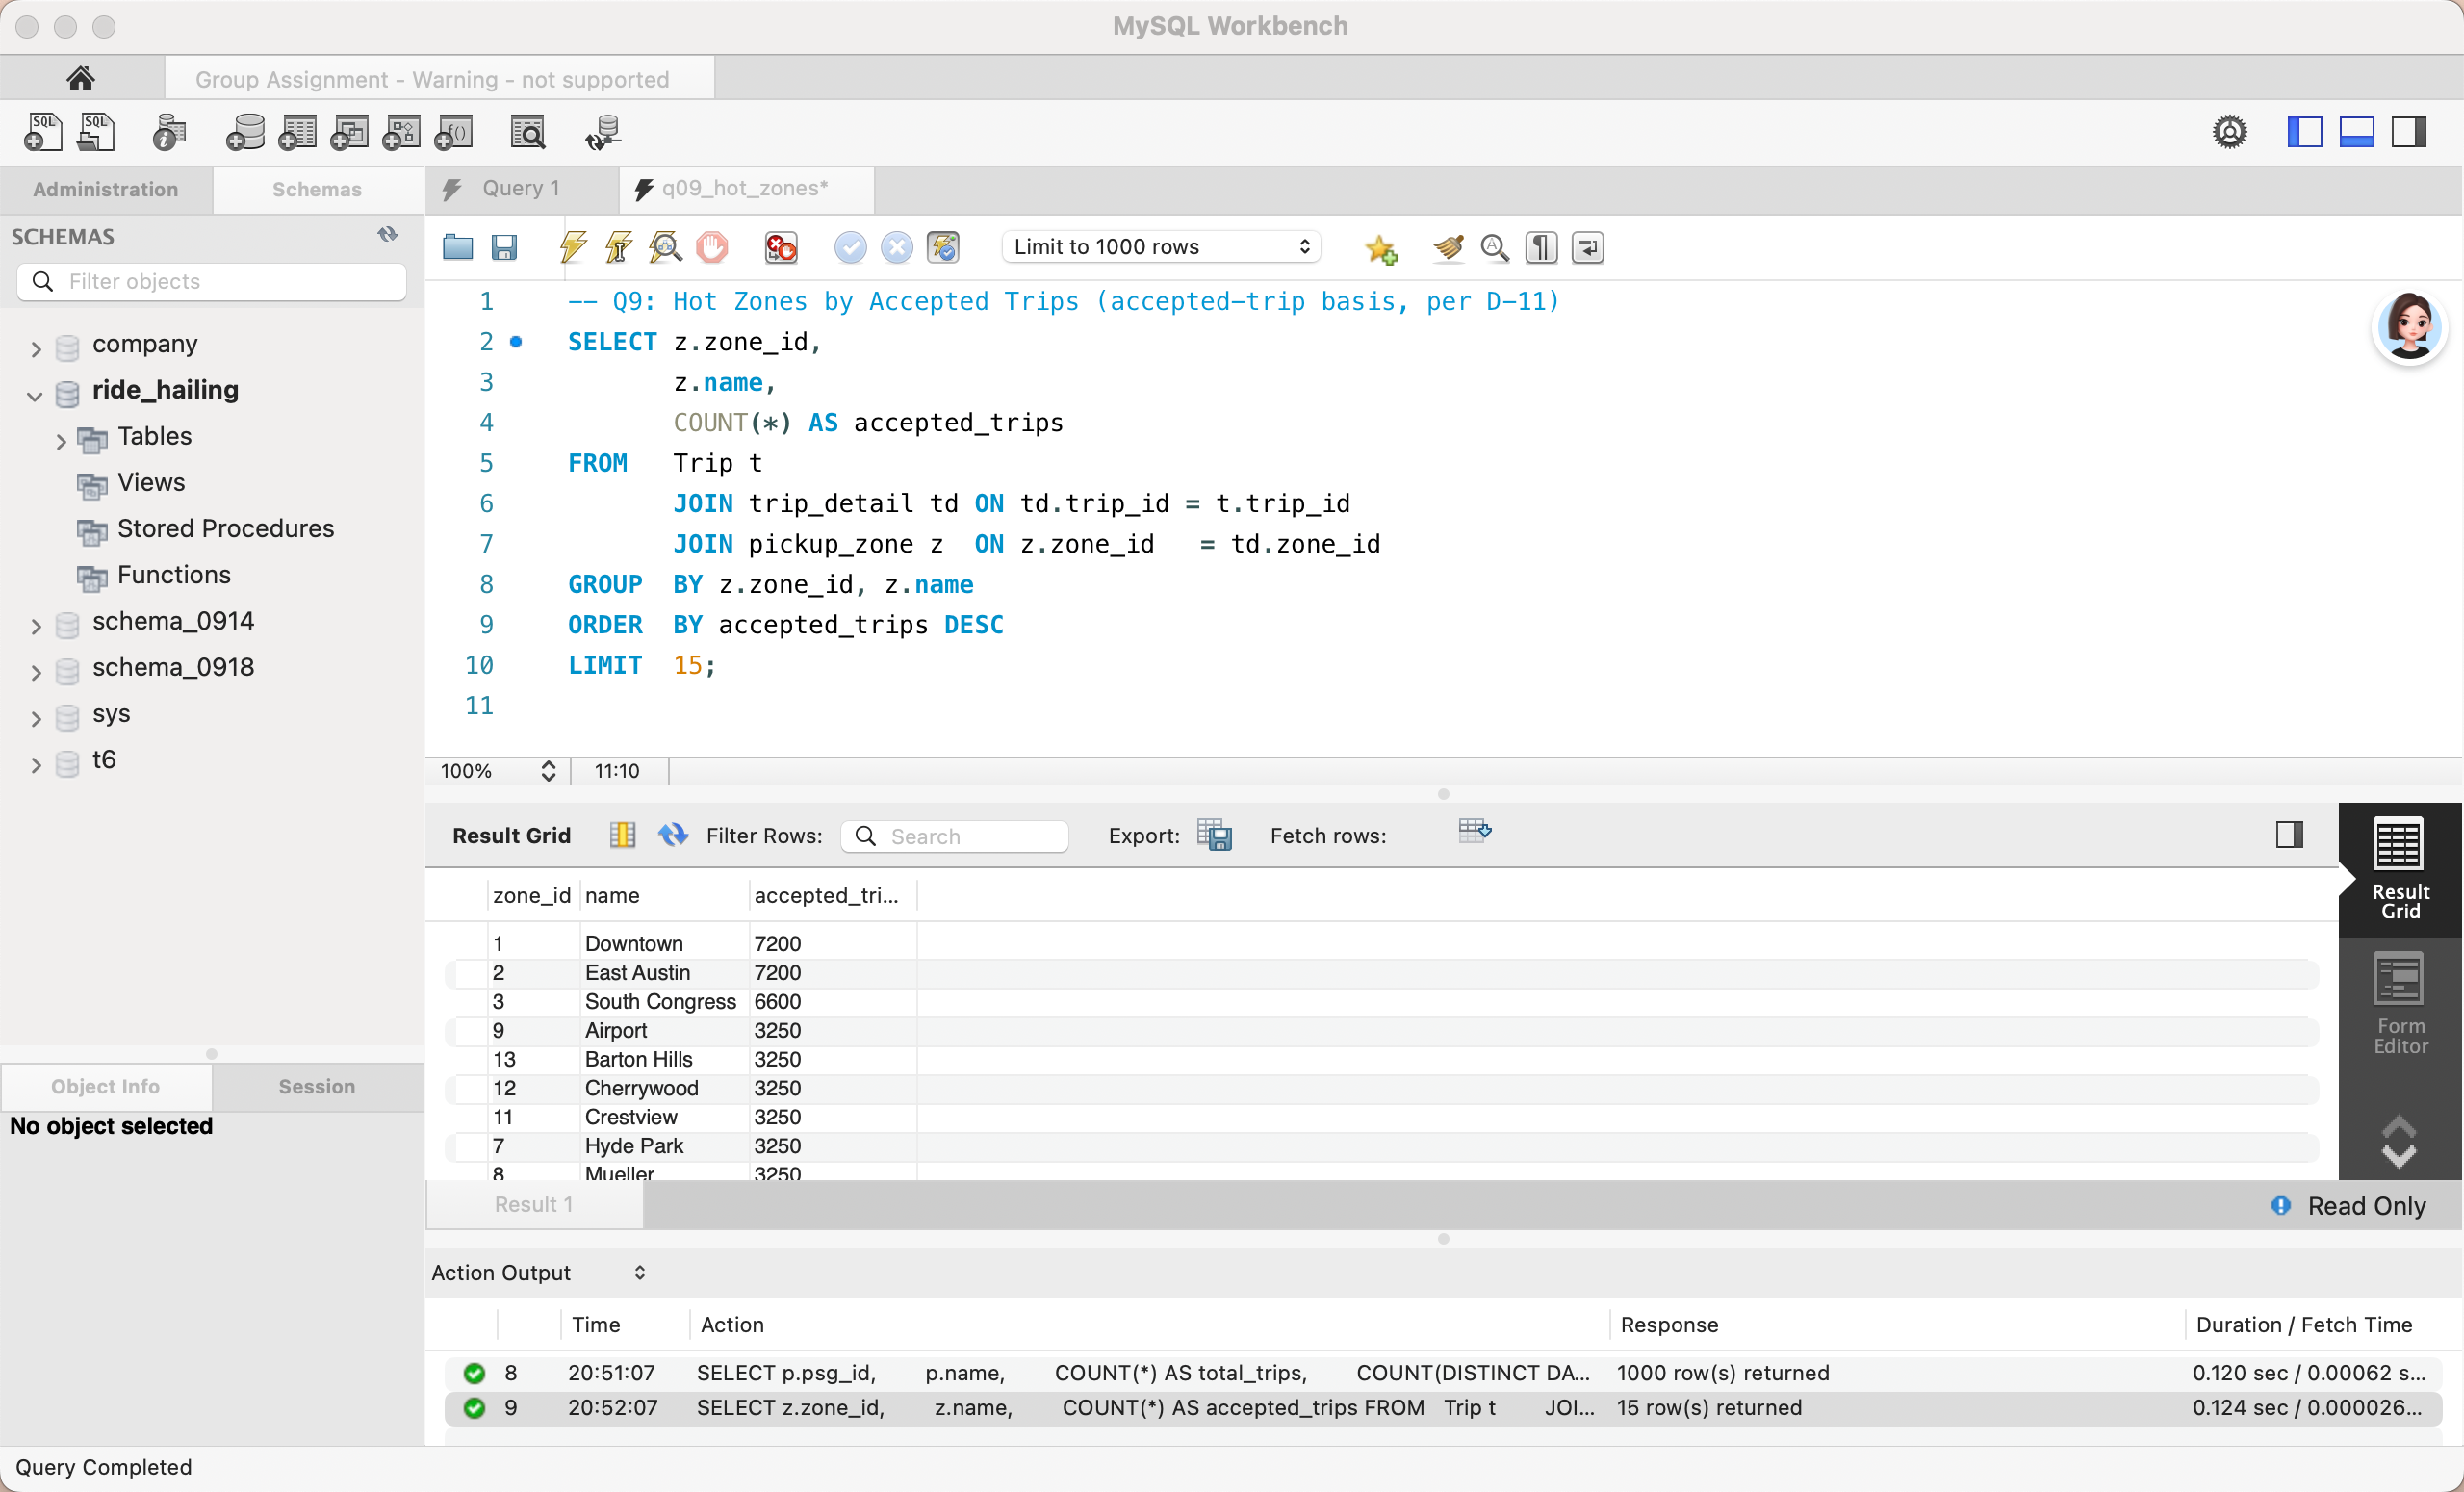
\includegraphics[width=0.72\textwidth]{q09_hot_zones_1029.png}
\caption{Q9 result: all 15 zones.}\label{fig:q09}
\end{figure}

\paragraph{Q10: Service tier $\times$ rating.}
The product-line comparison, restricted to completed trips (D-11). \texttt{COUNT(rating)} counts only non-NULL values, so it yields the rating coverage, while \texttt{AVG(rating)} ignores NULLs automatically --- the NULL semantics of Section~\ref{sec:er} in action. The tier mix matches calibration (95.1/3.7/0.9/0.3\%); average fare climbs from \$13.85 to \$41.62 ($\approx$3$\times$) across tiers while ratings stay flat around 4.85 with $\approx$90\% coverage --- premium products monetize without hurting satisfaction.

\begin{lstlisting}[caption={Q10 --- service tier vs.\ rating (completed only).}]
SELECT st.name AS tier,
       COUNT(*) AS completed_trips,
       ROUND(AVG(t.fare), 2) AS avg_fare,
       COUNT(td.rating) AS rated_trips,
       ROUND(COUNT(td.rating) / COUNT(*) * 100, 1) AS rating_cov_pct,
       ROUND(AVG(td.rating), 2) AS avg_rating
FROM Trip t
     JOIN trip_detail td  ON td.trip_id = t.trip_id
     JOIN service_tier st ON st.tier_id = td.service_tier_id
WHERE t.status = 'completed'
GROUP BY st.tier_id, st.name
ORDER BY completed_trips DESC;
\end{lstlisting}

\begin{figure}[h]\centering
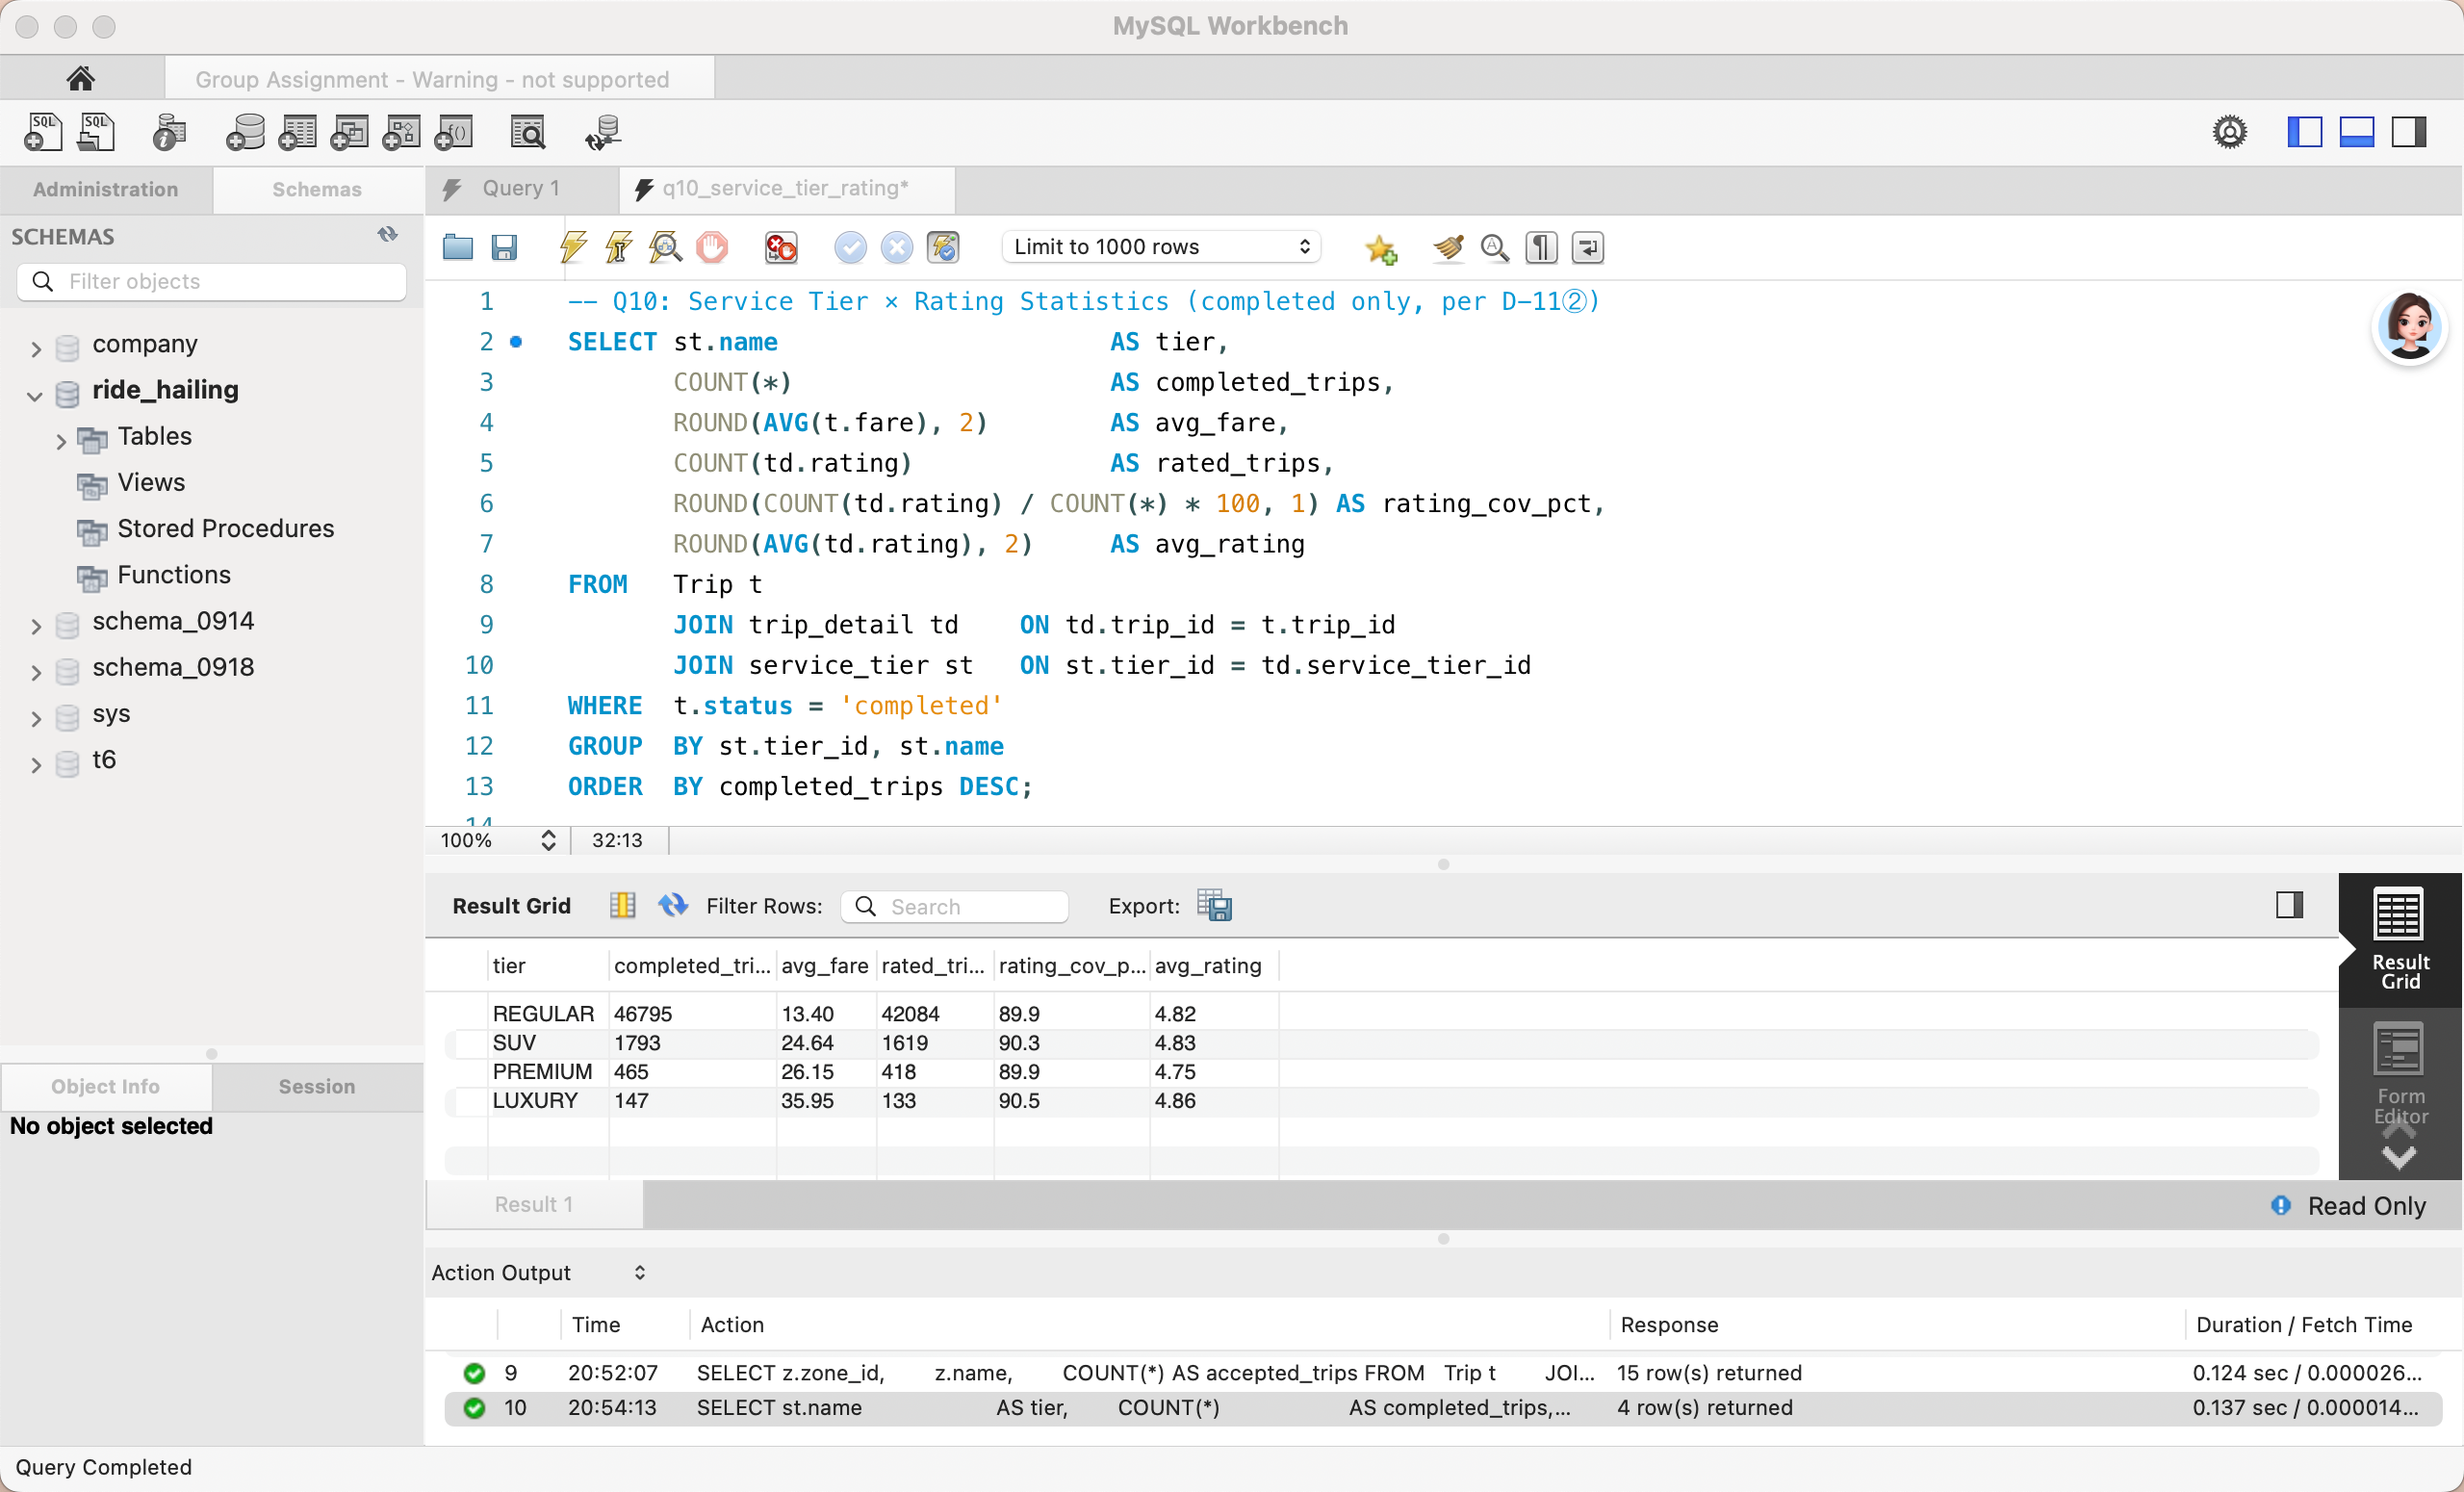
\includegraphics[width=0.72\textwidth]{q10_service_tier_rating_1029.png}
\caption{Q10 result across the four tiers.}\label{fig:q10}
\end{figure}

\subsection{Conceptual Q\&A}

\paragraph{Q1: Primary key vs.\ foreign key.}
A primary key identifies each row of a table: it is declared NOT NULL and UNIQUE and works like the address of a row, for instance \texttt{Passenger.psg\_id}. A foreign key is a column in a child table whose values must exist in the referenced key of the parent table; \texttt{Trip.psg\_id} is the example in our schema. The two work as a pair. Referential integrity fails the moment an orphan row appears, so MySQL rejects an insert such as \texttt{Trip(psg\_id=99999)} when passenger 99999 does not exist (error 1452), and it refuses to delete a parent row that is still referenced unless the schema declares CASCADE or SET NULL. We relied on this behaviour throughout the design. Every Trip points to a real Passenger and a real Driver, and \texttt{Payment.trip\_id}, which is NOT NULL, UNIQUE and a foreign key at once, also guarantees that a payment attaches to one real trip only --- this is how the 1:1 Trip--Payment relationship is actually implemented.

\paragraph{Q2: 1NF, 2NF and 3NF.}
Normalization removes redundancy level by level. First normal form asks that every cell hold one atomic value --- no lists such as ``morning peak, evening peak'' inside a single column. Second normal form removes partial dependencies: every non-key attribute must depend on the whole candidate key. This one comes for free in our design, because all five tables use single-column surrogate keys. Third normal form removes transitive dependencies, and this is where a concrete example helps. If we stored the plate directly in \texttt{Driver(driver\_id, name, vehicle\_id, plate)}, then plate would depend on vehicle\_id, which depends on the key --- a transitive chain. The chain brings three anomalies. Re-registering a vehicle would force updates to many driver rows, and missing one leaves the data inconsistent (update anomaly). Deleting the only driver of a vehicle would erase the plate as well (deletion anomaly). A vehicle with no driver yet could not be recorded at all (insertion anomaly). Splitting the table into \texttt{Driver} and \texttt{Vehicle} breaks the chain, which is exactly the structure we adopted.

\paragraph{Q3: INNER, LEFT and RIGHT JOIN.}
INNER JOIN keeps only the rows that match on both sides. LEFT JOIN keeps every row of the left table and fills the right-side columns with NULL where no match exists; RIGHT JOIN is the mirror image. The case where LEFT JOIN is genuinely needed is our per-driver activity report: ``list every driver with their completed-trip count, \emph{including} newly registered drivers who have completed zero trips''. An INNER JOIN quietly drops those zero-trip drivers, and the statistics would look better than reality. Two details make the LEFT JOIN version correct. The status filter belongs in the ON clause; placed in WHERE instead, it removes the NULL-extended rows and the join degenerates back into an INNER JOIN. And the count must be \texttt{COUNT(t.trip\_id)}, not \texttt{COUNT(*)}: for a driver without matches the former returns 0 while the latter counts the single NULL row as 1. We use this pattern for every per-driver report on the 60{,}000-trip table.

\paragraph{Q4: Subquery vs.\ JOIN.}
Take ``find the passengers who rode vehicle 3''. The JOIN formulation joins Passenger, Trip and Driver and removes duplicates with DISTINCT; the subquery formulation tests \texttt{psg\_id IN (SELECT ...)}. In principle the JOIN should win, because the optimizer can use the indexes on the join columns inside one execution plan, while older MySQL versions sometimes re-evaluated an IN subquery once per outer row. EXISTS is often the safest of the three, since it behaves as a semi-join and stops at the first match. In practice, though, MySQL 8 rewrites most IN and EXISTS forms into semi-joins, so the plans and the running times are often the same. One caveat: NOT IN is only safe when the subquery column is NOT NULL, which holds for \texttt{Payment.trip\_id}. Our Experiment~2 (Section~\ref{sec:eval}) shows exactly this: the three anti-join formulations return the same 1{,}442 rows with the same plan (\texttt{Extra: Not exists; Using index}), finishing within \_\_\_ ms of one another. Which formulation to pick is therefore a question for EXPLAIN, not for habit.
% TODO(D): 回填实验②三写法耗时（sec5 Table 对应行），删此行

\paragraph{Q5: ACID and concurrent payments.}
Atomicity: all writes in a transaction succeed together or leave no trace. Consistency: every committed state satisfies all declared constraints. Isolation: concurrent transactions never see each other's intermediate states. Durability: once committed, changes survive crash and restart. Now take a hypothetical wallet column with balance 100 and two concurrent \$50 payments. Both transactions read 100, both compute 50, and both write 50 back, so the final balance is 50 instead of 0 --- the classic lost update. One point deserves emphasis: the loss happens because the application reads first and updates later across two sessions; a single atomic \texttt{UPDATE ... SET balance = balance - 50} would not lose anything. The default REPEATABLE READ level does not save us either, since plain SELECTs are non-locking snapshot reads. The fix therefore has two layers. \texttt{SELECT ... FOR UPDATE} serializes the read-modify-write sequence at the isolation layer, while the UNIQUE constraint on \texttt{Payment.trip\_id} blocks a double payment of the same trip at the schema layer. Experiment~3 shows the failure and the fix live.

\paragraph{Q6: Indexes and B+ trees.}
An InnoDB index is a B+ tree. Internal nodes only route the search; the leaves hold keys with row pointers and are linked in key order, which is why range scans read sequentially. One lookup descends the tree in O(log n) steps instead of touching every row. That benefit has a price. Each index takes storage, every INSERT, UPDATE and DELETE has to maintain it, and the optimizer rarely picks an index on a low-selectivity column such as status on its own, so the practical rule is to index the high-selectivity columns that appear in WHERE, JOIN and ORDER BY, and to respect the leftmost-prefix order in composite indexes (for us: status equality first, start\_time range second). Foreign-key columns already get an index automatically (\texttt{Trip.psg\_id}, \texttt{driver\_id}) --- that is why our before/after comparison uses the composite (status, start\_time) as the baseline. Experiment~1 measured the effect: access type changed from ALL to range, estimated rows fell from 60{,}261 to 3{,}259, and actual time dropped from 16.6 ms to 0.46 ms thanks to a covering index.

\paragraph{Q7: GROUP BY, HAVING vs.\ WHERE.}
GROUP BY buckets the rows that survive WHERE into one output row per bucket, and the aggregates (COUNT, SUM, AVG, MIN, MAX) are computed inside each bucket; HAVING then decides which buckets survive. The difference from WHERE is timing. WHERE filters individual rows before grouping and cannot reference aggregates, while HAVING filters whole groups after aggregation and can --- putting an aggregate in WHERE is simply a syntax error. Our query ``months with at least 1{,}000 completed trips'' shows the division of labour: non-completed trips are discarded at the row level first (WHERE), the survivors are bucketed by month (GROUP BY), and only buckets reaching the threshold are kept (HAVING COUNT(*) $\ge$ 1000). The logical order FROM $\to$ WHERE $\to$ GROUP BY $\to$ HAVING $\to$ SELECT $\to$ ORDER BY $\to$ LIMIT explains why each filter sits where it sits, and the same three steps drive our Q6 and Q7 reporting queries, where filtering early also keeps each bucket small before the aggregation runs.

\paragraph{Q8: VIEW vs.\ STORED PROCEDURE.}
A view is a saved SELECT that behaves like a table. It stores no data of its own; the definition is expanded every time the view is queried. That makes it a good fit for reusing a complex query, hiding base tables behind a limited column set, and shielding callers from schema changes. A stored procedure is a different animal: a precompiled server-side program with parameters, control flow and DML, started with CALL. Its body contains semicolons, which is why the definition has to switch the DELIMITER first. The split in our project follows this line. The finance team gets \texttt{v\_completed\_revenue}, a view wrapping the daily completed-revenue query, while collections runs \texttt{sp\_check\_unpaid(24)}, a procedure that takes the overdue threshold as a parameter and is invoked with CALL. A stored FUNCTION sits between the two when a scalar return value is enough. Put simply, a view is queried and a procedure is run.
